\setchapterimage{monoblocks_roux_cropped}
\setchapterpreamble[u]{\margintoc}
\chapter{Monoblocks}\label{Chapter3}\labch{Chapter3}

In order to assess the behaviour of H in the divertor, component-level simulations of monoblocks are required.

This chapter will focus on simulating H transport in ITER-like monoblocks.

\refsec{model description} will describe the model geometry, the boundary conditions as well as the materials and trap properties.
Then, \refsec{simulation simplifications} will review the simplifications that can be brought to the model to reduce the computation time.
Finally, with these simplifications, a parametric study will be performed and a behaviour law linking the monoblock H inventory to the exposure conditions will be determined in \refsec{influence of exposure conditions}.

\section{Model description}\labsec{model description}

The monoblock geometry is described on \reffig{monoblock geometry}.
The boundary conditions for the heat transfer problem are described in \refeq{bc thermal monoblock} and those for the hydrogen transport problem are described in \refeq{bc H transport monoblock}.
An instantaneous recombination is assumed on the poloidal and toroidal gaps and at the plasma facing surface.
This assumption is consistent with the high recombination coefficient measured by Ogorodnikova \sidecite{ogorodnikova_recombination_2019} compared to Anderl's coefficient \sidecite{anderl_deuterium_1992}.

The materials properties (diffusivity, solubility, and thermal conductivity, density and heat capacity) are described in \reftab{materials properties monoblock} and plotted on \reffig{properties monoblock}.
Finally, the traps properties are described in \reftab{traps monoblock}.

\begin{figure}
    \begin{overpic}[width=\linewidth]{Figures/Chapter3/monoblocks/interface_condition/iter case/monoblock_sketch.pdf}
        \put(42, 5){\SI{28}{mm}}
        \put(97, 50){\SI{28}{mm}}
        \put(10, 32){\SI{13.5}{mm}}
        \put(42, 62){ \diameter \SI{12}{mm}}
        \put(42, 71){ \diameter \SI{15}{mm}}
        \put(42, 76){ \diameter \SI{17}{mm}}
        \put(20, 80){\large$\Gamma_\mathrm{top}$}
        \put(4, 60){\large$\Gamma_\mathrm{toroidal}$}
        \put(78, 60){\large$\Gamma_\mathrm{toroidal}$}
        \put(40, 41){\large$\Gamma_\mathrm{coolant}$}
    \end{overpic}
    \caption{ITER monoblock geometry showing W armour \cruleme[grey]{0.3cm}{0.3cm}, Cu interlayer \cruleme[orange]{0.3cm}{0.3cm}, CuCrZr alloy cooling pipe  \cruleme[yellow]{0.3cm}{0.3cm}. The monoblock thickness is \SI{12}{mm}.}
    \labfig{monoblock geometry}
\end{figure}

\begin{subequations}
    \begin{align}
    -\lambda \nabla T \cdot \mathbf{n} &=\varphi_\mathrm{heat} \quad  &\text { on } \Gamma_\mathrm{top}\\
    -\lambda \nabla T\cdot \mathbf{n} &= -h \cdot \left(T_\mathrm{coolant} - T\right)\quad &\text { on } \Gamma_\mathrm{coolant}
    \end{align}
    \labeq{bc thermal monoblock}
\end{subequations}
where $T_\mathrm{coolant} = \SI{323}{K}$ and $h = \SI{70000}{W.m^{-2}.K^{-1}}$.

\begin{subequations}
    \begin{align}
    c_\mathrm{m} &=  \frac{\varphi_\mathrm{imp} R_p}{D} \quad &\text { on } \Gamma_\mathrm{top}\\
    -D \nabla c_\mathrm{m} \cdot \mathbf{n} &= K_\mathrm{r, \, CuCrZr} \cdot c_\mathrm{m}^{2} \quad &\text { on } \Gamma_\mathrm{coolant} \\
    c_\mathrm{m} &=  0 \quad &\text { on } \Gamma_\mathrm{toroidal} \text{  and  } \Gamma_\mathrm{poloidal} \\
    \end{align}
    \labeq{bc H transport monoblock}
\end{subequations}
where $K_\mathrm{r, \, CuCrZr} = 2.9 \times 10^{-14}\cdot \exp{(-1.92/(k_B\cdot T))}$ the recombination coefficient of the copper alloy (in vacuum) expressed in \si{m^4.s^{-1}} \sidecite{anderl_deuterium_1999}.

\begin{table*}
    \centering
    \begin{tabular}{p{1.7cm}  R{3cm}  R{3cm}  R{1.8cm}  R{1cm} R{1.8cm}  R{1cm}}
         & \multicolumn{2}{c}{Thermal properties} & \multicolumn{4}{c}{Hydrogen transport properties}\\
        \hline
        Material & $\rho \cdot C_p \newline(\si{J.K^{-1}.m^{-3}})$ & $\lambda \newline(\si{W.m^{-1}.K^{-1}})$ & $D_0 \newline(\si{m^2.s^{-1}})$ & $E_D \newline(\si{eV})$ & $S_0 \newline(\si{m^{-3}.Pa^{-0.5}})$ & $E_\mathrm{S} \newline(\si{eV})$\\
        \hline
        \\
        W \cite{frauenfelder_solution_1969,fernandez_hydrogen_2015}& %
        $5.1\times 10^{-6} \cdot T^3 \newline - 8.3\times 10^{-2}\cdot T^2 \newline + 6.0 \times 10^{2}\cdot T \newline +2.4\times 10^6$ &%
        $-7.8\times 10^{-9}\cdot T^3 \newline %
        +5.0\times 10^{-5}\cdot T^2 \newline%
        -1.1\times 10^{-1} \cdot T \newline%
        +1.8\times 10^{2}$ &%
        $1.9\times 10^{-7}$ & 0.20 &%
        $1.87\times 10^{24}$ & 1.04\\
        \\
        Cu \cite{reiter_compilation_1996}&%
        $1.7\times 10^{-4}\cdot T^3\newline %
        +6.1\times 10^{-2}\cdot T^2\newline %
        +4.7\times 10^2\cdot T\newline %
        +3.5\times 10^6$ &%

        $-3.9\times 10^{-8}\cdot T^3\newline %
        +3.8\times 10^{-5}\cdot T^2\newline %
        -7.9\times 10^{-2}\cdot T\newline %
        +4.0\times 10^2 $&%

        $6.6\times 10^{-7}$ &%
        0.39&%
        $3.14\times 10^{24}$ & 0.57\\
        \\
        CuCrZr \cite{serra_hydrogen_1998}& %
        $-1.8\times 10^{-4}\cdot T^3 \newline %
        +1.5\times 10^{-1}\cdot T^2\newline %
        +6.2\times 10^2\cdot T\newline %
        +3.5\times 10^6$ &%

        $5.3\times 10^{-7}\cdot T^3\newline %
        -6.5\times 10^{-4}\cdot T^2\newline %
        +2.6\times 10^{-1}\cdot T\newline %
        +3.1\times 10^2$ & %

        $3.9\times 10^{-7}$ & %
        0.42&%
        $4.28\times 10^{23}$ & 0.39\\
        \\
        \\
    \end{tabular}
    \caption{Materials properties used in the simulations. Thermal properties are fitted from ANSYS. $T$ is the temperature in \si{K}.}
    \labtab{materials properties monoblock}
\end{table*}

\begin{figure}
    \centering
    \begin{subfigure}{\linewidth}
        \centering
        \includegraphics[width=\linewidth]{Figures/Chapter3/monoblocks/interface_condition/iter case/thermal_prop.pdf}
        \caption{Thermal properties.}
    \end{subfigure}
    \begin{subfigure}{\linewidth}
        \centering
        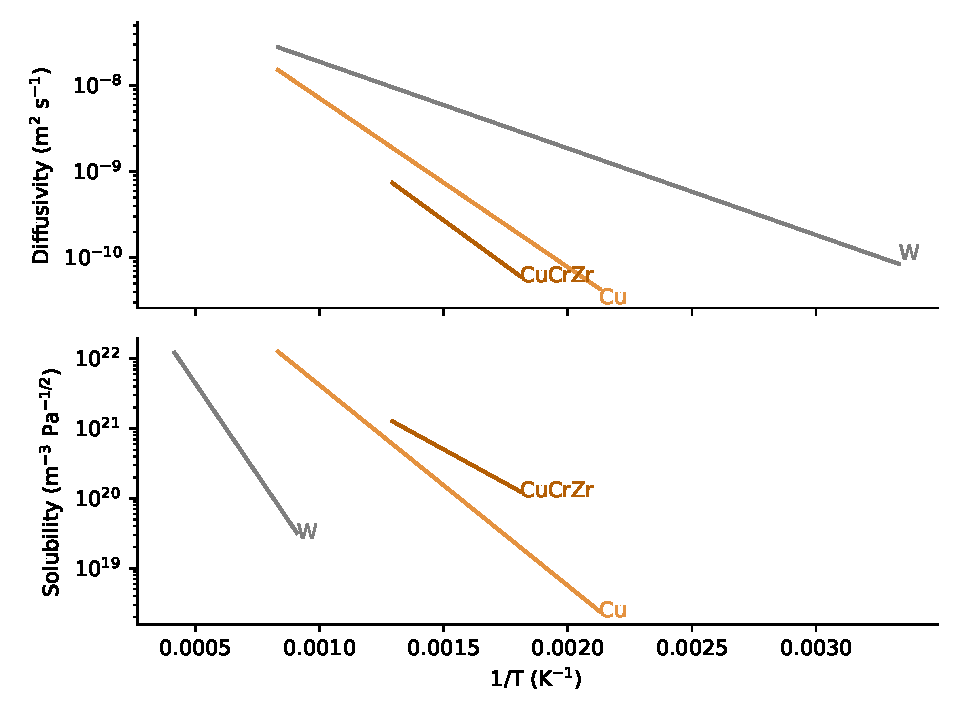
\includegraphics[width=\linewidth]{Figures/Chapter3/monoblocks/monoblock_H_transport_properties.pdf}
        \caption{H transport properties.}
    \end{subfigure}
    \caption{Material properties used in the simulations \cite{frauenfelder_solution_1969, reiter_compilation_1996, serra_hydrogen_1998, aiello_hydrogen_2002}.}
    \labfig{properties monoblock}
\end{figure}

\begin{table*}
    \centering
    \begin{tabular}{L{1.5cm} L{1.5cm} R{1.7cm} R{1.1cm} R{1.6cm} R{1.1cm} R{1.9cm}}
         & Material & $k_0 (\si{m^3.s^{-1}})$ &  $E_k (\si{eV})$ & $p_0 (\si{s^{-1}})$ & $E_p (\si{eV})$ & $n_i (\si{at.fr.})$ \\
        \hline
        \\
        Trap 1 & W & $8.96 \times 10^{-17}$ & 0.2 & $1 \times 10^{13}$& 0.87 & $1.1 \times 10^{-3}$ \\
        \\
        Trap 2 & W & $8.96 \times 10^{-17}$ & 0.2 & $1 \times 10^{13}$& 1.00 & $4.0 \times 10^{-4}$ \\
        \\
        Trap 3 & Cu & $6.0 \times 10^{-17}$ & 0.39 & $8.0 \times 10^{13}$ & 0.50 &$5.0 \times 10^{-5}$\\
        \\
        Trap 4 & CuCrZr & $1.2\times 10^{-16}$ & 0.42 & $8.0 \times 10^{13}$ & 0.85 &$5.0 \times 10^{-5}$\\
        \\
    \end{tabular}
    \caption{Traps properties used in the simulations \cite{hodille_macroscopic_2015, dolan_assessment_1994}.}
    \labtab{traps monoblock}
\end{table*}

\section{Simulation simplifications}\labsec{simulation simplifications}

\subsection{Thermal behaviour}\labsec{monoblock thermal behaviour}
Steady-state heat transfer simulations were performed with FESTIM with varying heat fluxes $\varphi_\mathrm{heat}$.
With $\varphi_\mathrm{heat} = \SI{1}{MW.m^{-2}}$, the surface temperature of the monoblock was found to be around \SI{400}{K} (see \reffig{T field 1 MW}) whereas with $\varphi_\mathrm{heat} = \SI{10}{MW.m^{-2}}$ the surface was around \SI{1400}{K} (see \reffig{T field 10 MW}).

\begin{figure*} [h!]
    \centering
    \begin{subfigure}{0.4\linewidth}
        \centering
        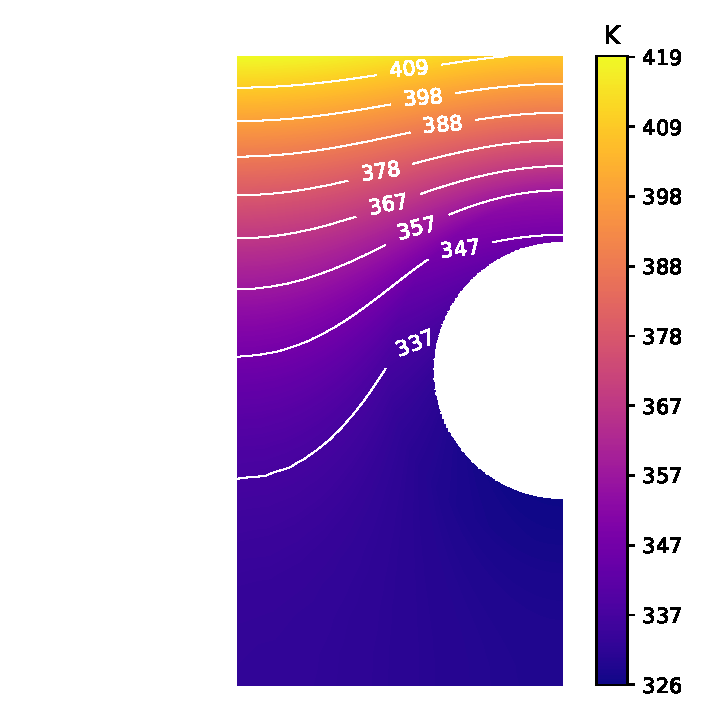
\includegraphics[width=\linewidth]{Figures/Chapter3/monoblocks/parametric_study/T_1e6.pdf}
        \caption{Temperature field with $\varphi_\mathrm{heat} = \SI{1}{MW.m^{-2}}$.}
        \labfig{T field 1 MW}
    \end{subfigure}%
    \begin{subfigure}{0.4\linewidth}
        \centering
        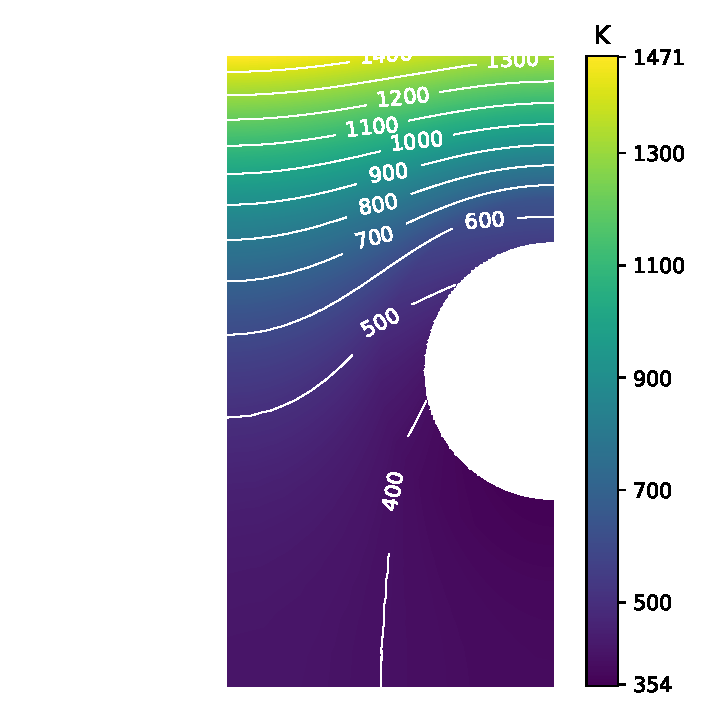
\includegraphics[width=\linewidth]{Figures/Chapter3/monoblocks/parametric_study/T_1e7.pdf}
        \caption{Temperature field with $\varphi_\mathrm{heat} = \SI{10}{MW.m^{-2}}$.}
        \labfig{T field 10 MW}
    \end{subfigure}
    \begin{subfigure}{0.7\linewidth}
        \centering
        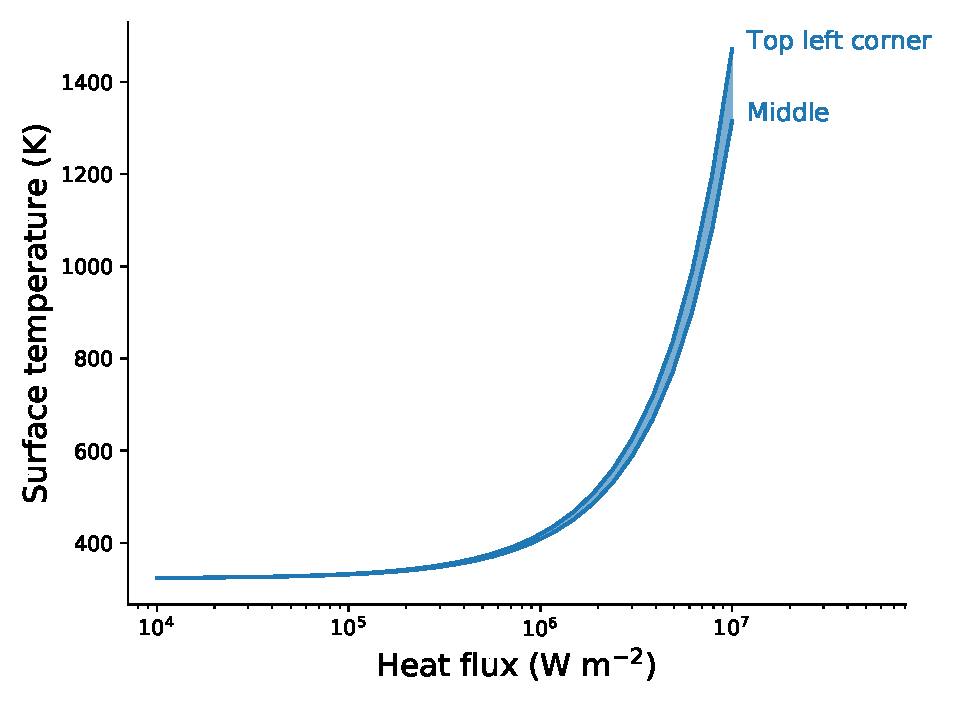
\includegraphics[width=\linewidth]{Figures/Chapter3/monoblocks/parametric_study/temperature_phi_H.pdf}
        \caption{Evolution of surface temperature as a function of heat flux.}
        \labfig{surface temperature as a function of heat flux}
    \end{subfigure}
    \caption{Thermal behaviour of the monoblock.}
\end{figure*}

The average surface temperature $T_\mathrm{surface}$ therefore increases linearly with the heat load and can be fitted by \refeq{thermal behaviour law} (see \reffig{surface temperature as a function of heat flux}).
\begin{equation}
    T_\mathrm{surface} = 1.1 \times 10^{-4} \cdot \varphi_\mathrm{heat} + T_\mathrm{coolant}
    \labeq{thermal behaviour law}
\end{equation}

This was found to be in very good agreement with experimental measurements performed in \sidecite{hirai_use_2016}.
Using a mean surface temperature had low influence on the hydrogen transport results compared to a non-homogeneous surface temperature that could be obtained with a heat flux condition since surface temperature gradient was low compared to the one between the top surface and the cooling surface.

\subsection{Influence of dimensionality}\labsec{influence of dimensionality}

The first simplification that can be done is the dimensionality.
A full 3D simulation would be the most accurate, but also the most expensive in terms of computation time (partly because more cells are required for the same spatial discretisation as seen on \reffig{monoblock meshes}).
Conversely, 1D simulations are faster to run, but are less accurate.
This is sometimes referred as the \textit{curse of dimensionality}.

\begin{figure}
    \centering
    \begin{subfigure}{0.27\linewidth}
        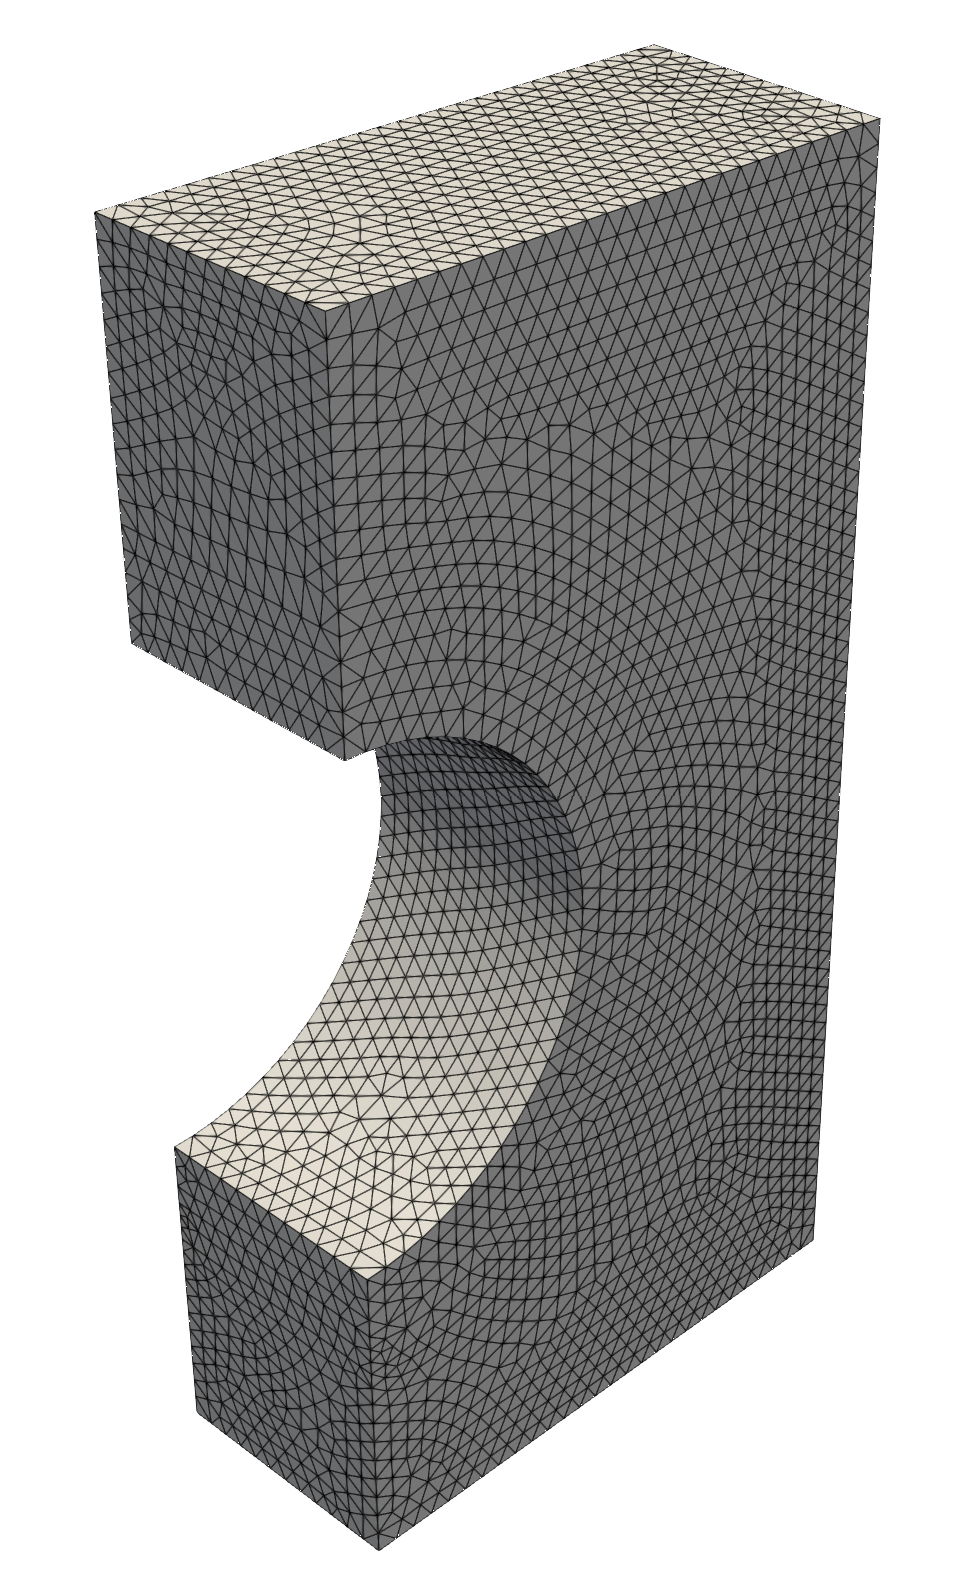
\includegraphics[width=\linewidth]{Figures/Chapter3/monoblocks/mesh_3d.png}
        \caption{3D mesh.}
    \end{subfigure}%
    \begin{subfigure}{0.73\linewidth}
        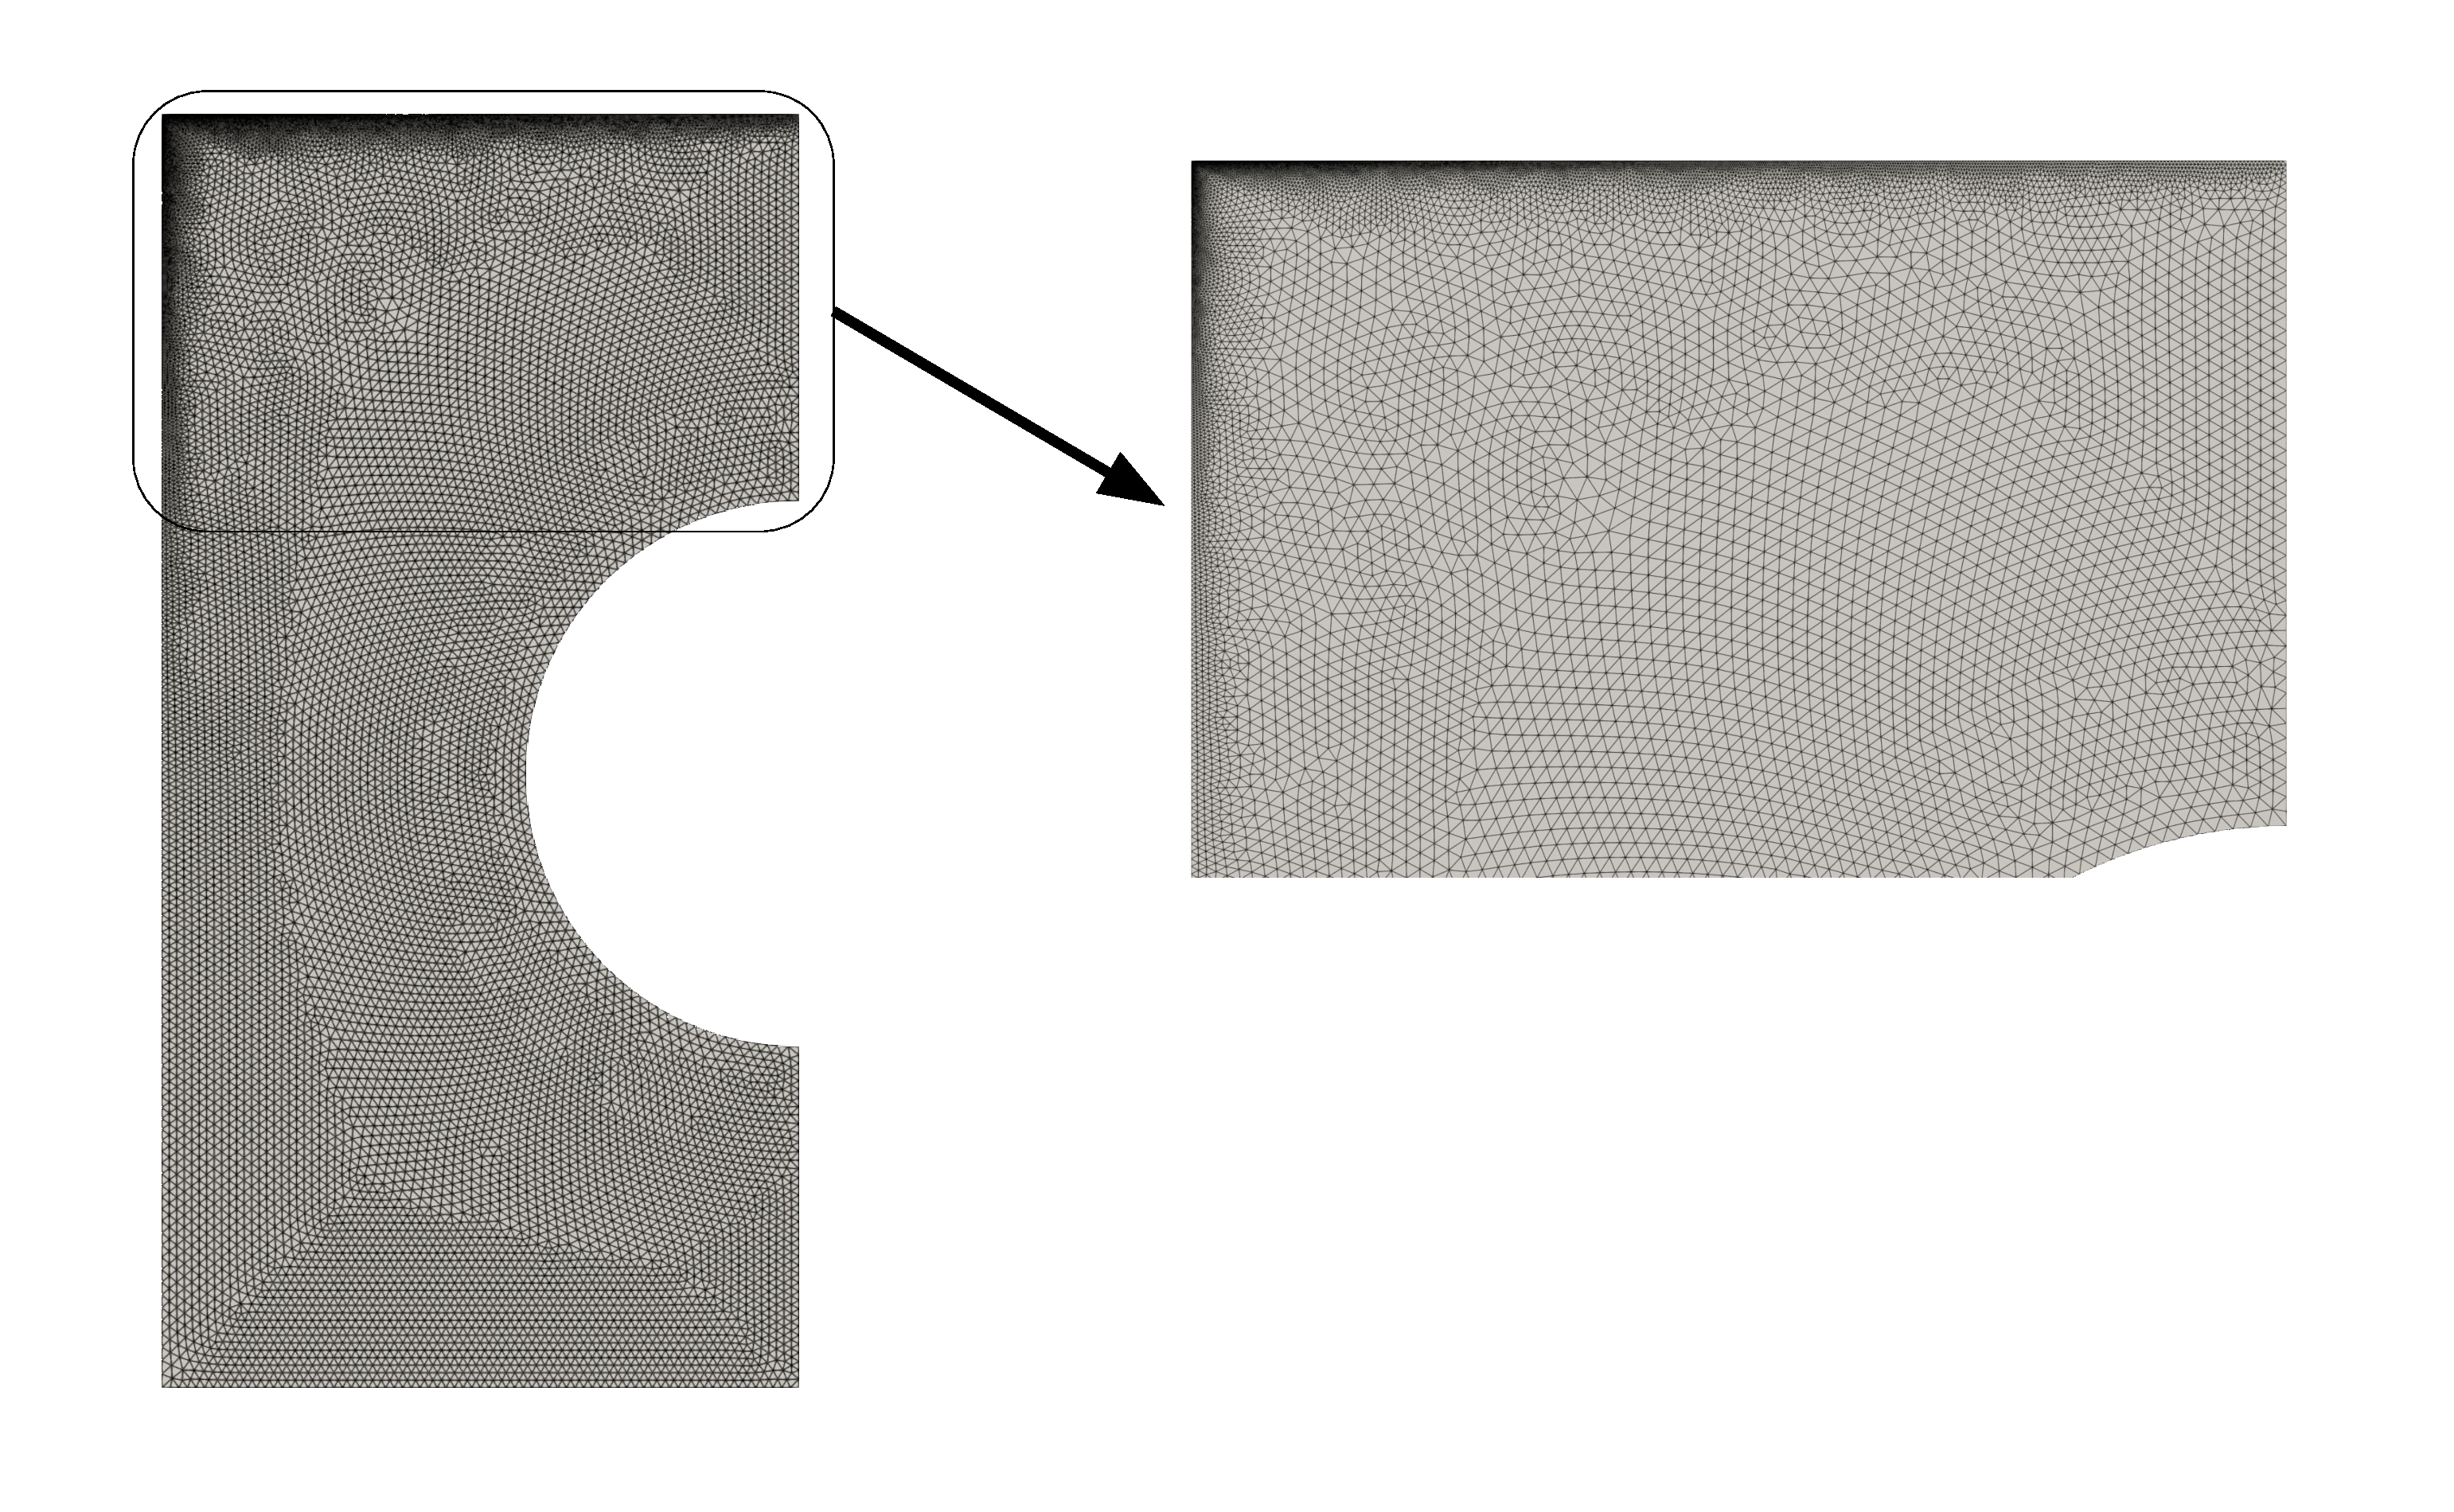
\includegraphics[width=\linewidth]{Figures/Chapter3/monoblocks/mesh_2d.pdf}
        \caption{2D mesh.}
    \end{subfigure}
    \caption{Meshes used for the monoblock simulations.}
    \labfig{monoblock meshes}
\end{figure}

A 2D approximation assumes the solution is independent of the poloidal direction.
The hydrogen inventory is obtained by:

\begin{equation}
    \mathrm{inv} = e \int_\Omega (c_\mathrm{m} + \sum c_\mathrm{t,\, i}) \, dS
\end{equation}
where $e$ is the monoblock thickness.

Similarly, the 1D approximation assumes the solution is independent of both the poloidal and the toroidal direction (see \reffig{dimension approximations monoblock}).
It also cannot capture the full geometry of the monoblock as it would assume Cu and CuCrZr slabs instead of hollow cylinders.
The hydrogen inventory is obtained by:

\begin{equation}
    \mathrm{inv} = e \, L \int_\Omega (c_\mathrm{m} + \sum c_\mathrm{t,\, i}) \, dl
\end{equation}
where $L$ is the monoblock width.

\begin{figure}
    \centering
    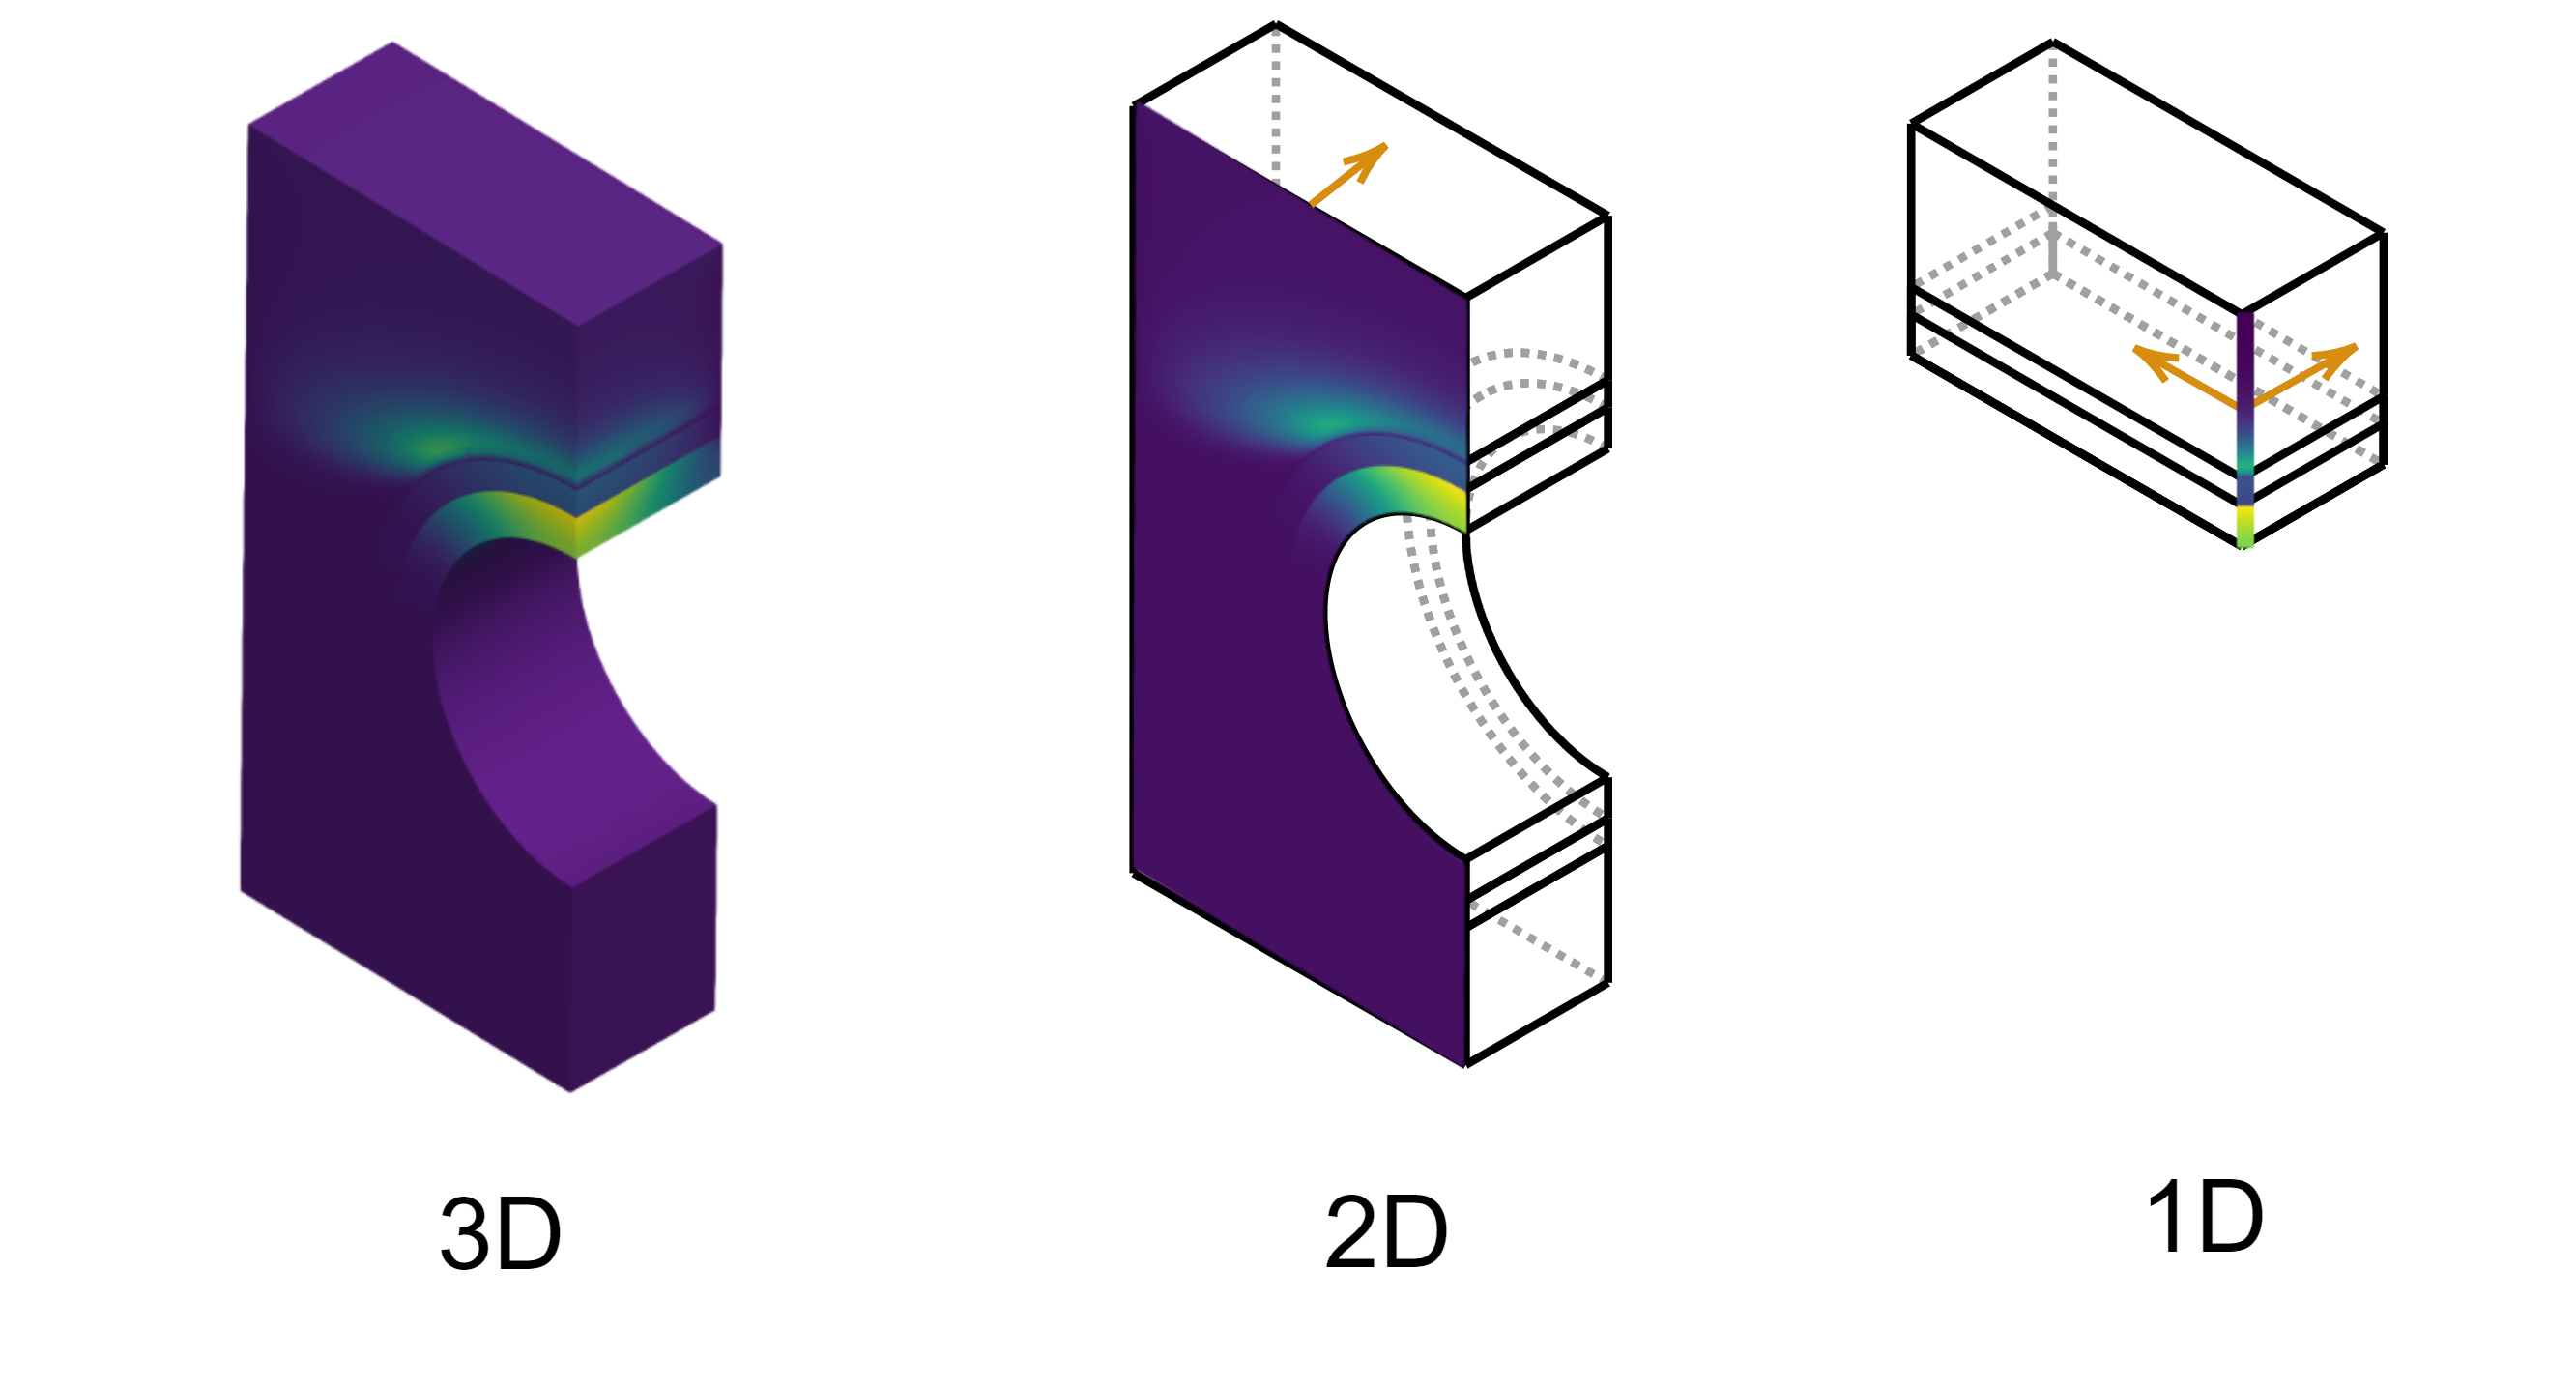
\includegraphics[width=\linewidth]{Figures/Chapter3/monoblocks/dimension_approximation.png}
    \caption{Representation of the 2D and 1D approximations on a monoblock geometry. The arrows represent geometry independencies.}
    \labfig{dimension approximations monoblock}
\end{figure}

Monoblocks simulations were run in 1D, 2D, and 3D and the inventory was computed for each case (see \reffig{monoblock inventories 1d 2d 3d}).
Both the 1D and 2D approximations overestimate the inventory compared to the 3D reference, these approximations are therefore conservative.
It should however be noticed that, when neglecting the recombination on the poloidal gap (i.e.\ assuming hydrogen cannot desorb from this surface), the 2D approximation is strictly equivalent to the 3D reference (see \refch{DEMO monoblocks}).
For these reasons, the 2D approximation will be employed in the following sections as it is the best compromise between accuracy and computational time.

\begin{figure}
    \centering
    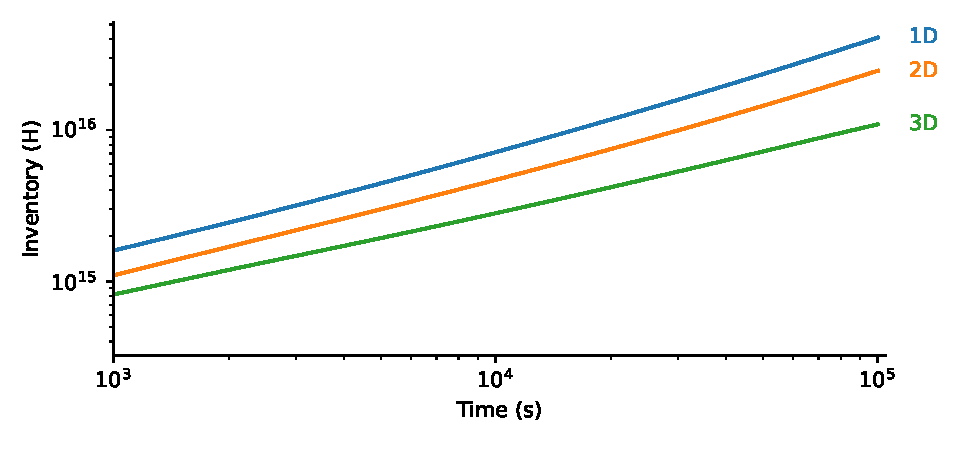
\includegraphics[width=\linewidth]{Figures/Chapter3/monoblocks/3D_monoblocks/comparison_inventory_1d_2d_3d.pdf}
    \caption{Comparison of monoblock inventories for the 1D, 2D approximations and the 3D case.}
    \labfig{monoblock inventories 1d 2d 3d}
\end{figure}

\subsection{Influence of interface condition}\labsec{influence of interface conditions}
\begin{figure}
    \centering
    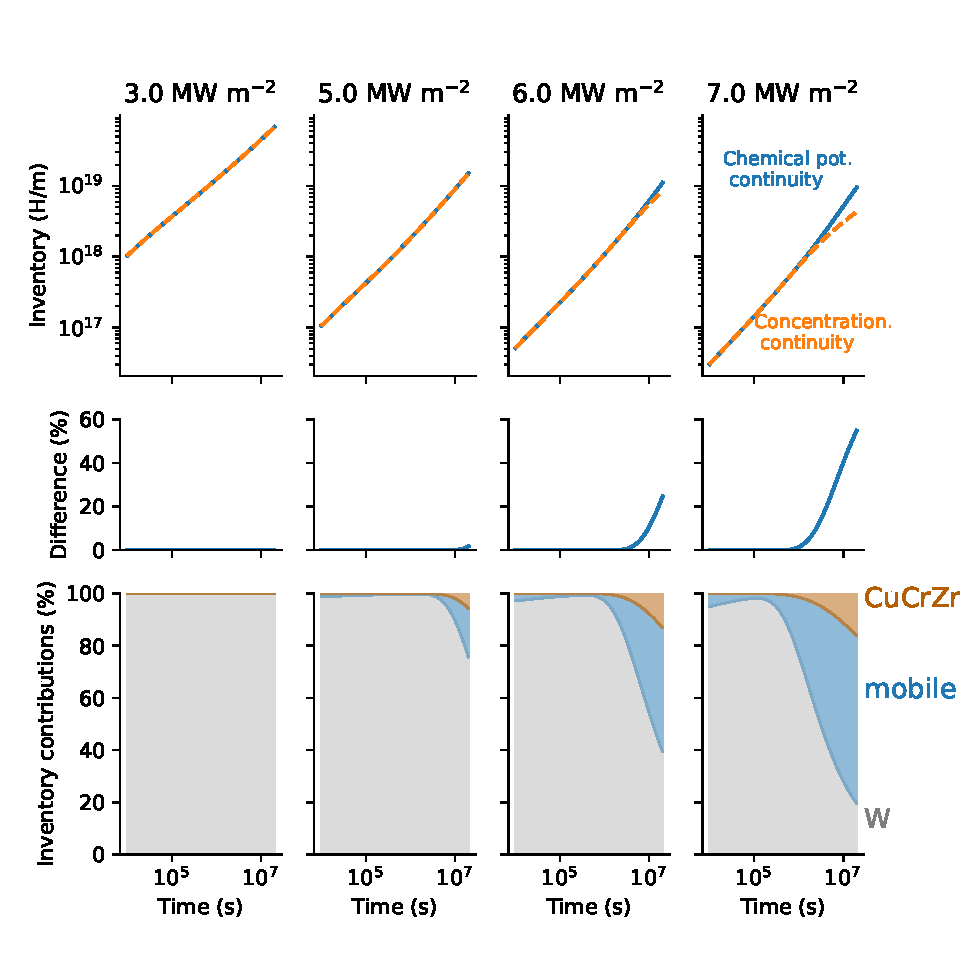
\includegraphics[width=\linewidth]{Figures/Chapter3/monoblocks/interface_condition/difference_w_wo_chemical_pot.pdf}
    \caption{Influence of continuity of chemical potential on the monoblock hydrogen inventory. The bottom plot shows the contribution of the trapped hydrogen in W, Cu and CuCrZr as well as the total mobile hydrogen for the case with continuity of chemical potential.}
    \labfig{influence of chemical potential on monoblock inventory}
\end{figure}


\begin{figure}
    \centering
    \begin{subfigure}{0.5\linewidth}
        \centering
        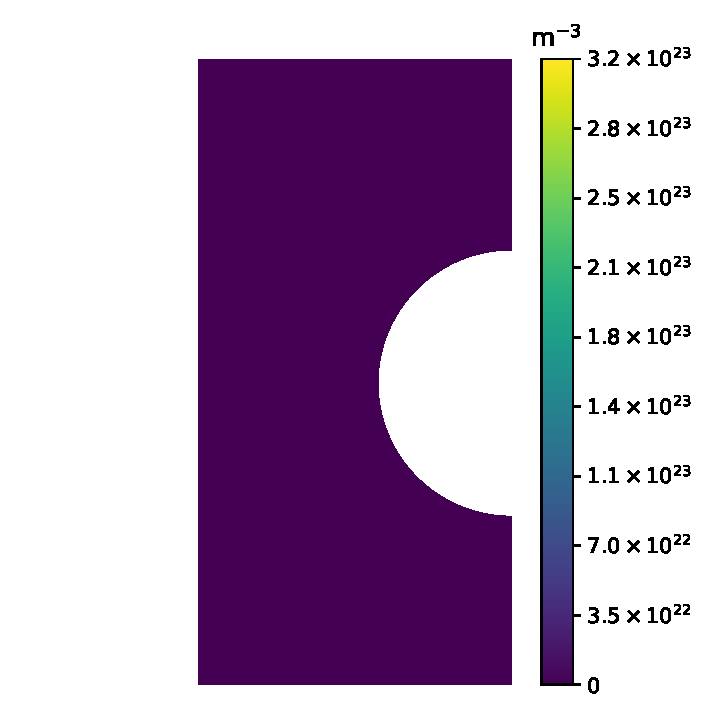
\includegraphics[width=\linewidth]{Figures/Chapter3/monoblocks/interface_condition/iter case/mobile_concentration.pdf}
        \caption{$c_\mathrm{m}$ (continuity of $c_\mathrm{m}$).}
    \end{subfigure}%
    \begin{subfigure}{0.5\linewidth}
        \centering
        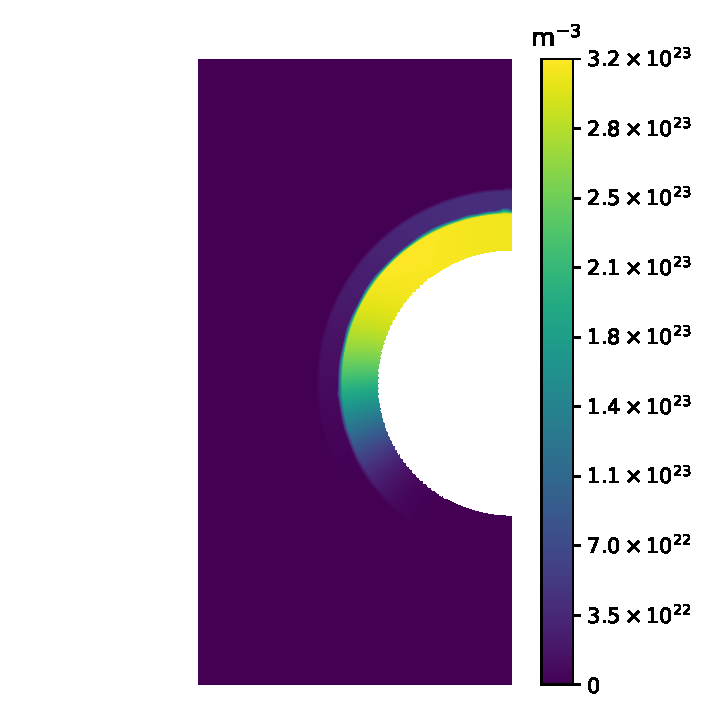
\includegraphics[width=\linewidth]{Figures/Chapter3/monoblocks/interface_condition/iter case/mobile_chemical_pot.pdf}
        \caption{$c_\mathrm{m}$ (continuity of chemical potential).}
    \end{subfigure}
    \begin{subfigure}{0.5\linewidth}
        \centering
        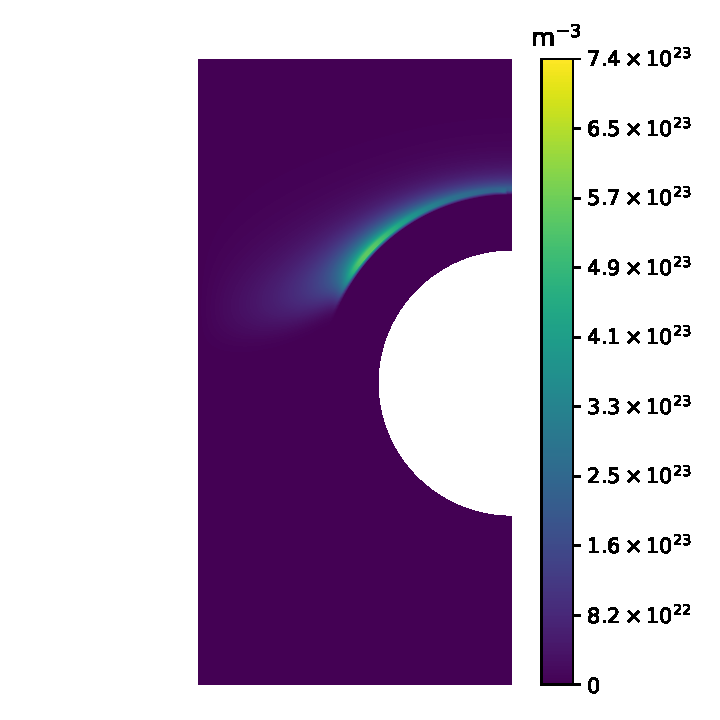
\includegraphics[width=\linewidth]{Figures/Chapter3/monoblocks/interface_condition/iter case/retention_concentration.pdf}
        \caption{Retention (continuity of $c_\mathrm{m}$).}
    \end{subfigure}%
    \begin{subfigure}{0.5\linewidth}
        \centering
        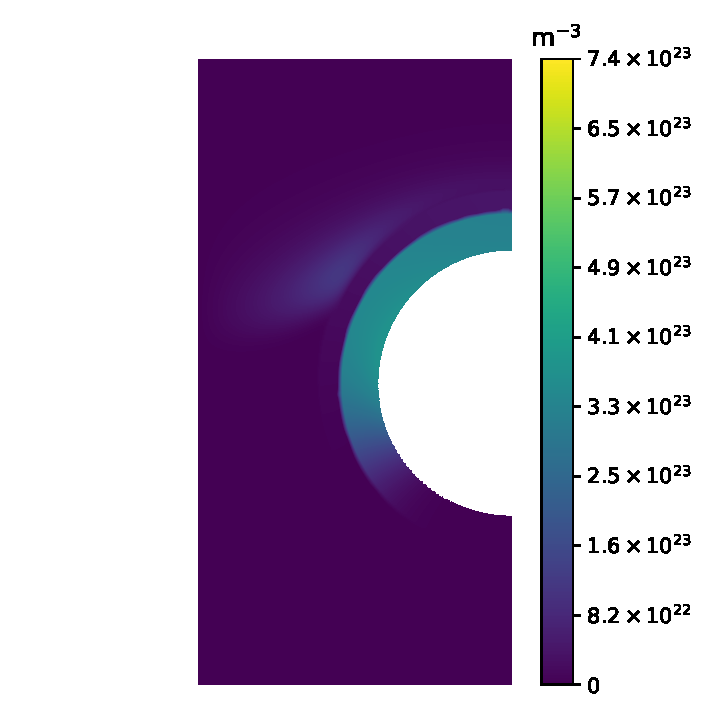
\includegraphics[width=\linewidth]{Figures/Chapter3/monoblocks/interface_condition/iter case/retention_chemical_pot.pdf}
        \caption{Retention (continuity of chemical potential).}
    \end{subfigure}
    \caption{Concentration fields at $t=\SI{2e7}{s}$, $\varphi_\mathrm{heat} = \SI{7}{MW.m^{-2}}$.}
    \labfig{concentration fields w/wo chemical potential}
\end{figure}

As monoblocks are made of several materials (tungsten, copper and CuCrZr), the continuity of chemical potential across interfaces results in a mobile concentration jump (see \refsec{conservation of chemical potential}).
However, the problem could be simplified if, instead of ensuring the continuity of chemical potential, one ensured the continuity of mobile concentration across interfaces.
Indeed, this would allow getting rid of one equation and therefore reduce the computational time.
But is this simplification valid?

To verify its validity, 2D monoblock simulations are performed with chemical potential continuity (see \refeq{c/s conservation}) or mobile concentration continuity and the temporal evolution of the inventory was computed.
The implanted flux $\varphi_\mathrm{imp}$ was fixed to \SI{1.0e21}{m^{-2}.s^{-1}} and the heat flux $\varphi_\mathrm{heat}$ varied from \SI{3.0}{MW.m^{-2}} to \SI{7.0}{MW.m^{-2}}.

For the low flux cases (\SI{3}{MW.m^{-2}} and \SI{5}{MW.m^{-2}}), no difference was found (see \reffig{influence of chemical potential on monoblock inventory}).
For the case at \SI{6}{MW.m^{-2}}, differences start to appear after \SI{3e6}{s} (\SI{7e5}{s} at \SI{7}{MW.m^{-2}}).
After \SI{2e7}{s} of continuous exposure, the absolute difference at \SI{6}{MW.m^{-2}} was 25 \% and 55 \% at \SI{7}{MW.m^{-2}}.

This time of appearance of differences corresponds to the time required for the hydrogen to migrate up to the W/Cu interface.
This is explained by the high solubility ratio between W, Cu and CuCrZr leading to a higher concentration of mobile particles in CuCrZr (see \reffig{concentration fields w/wo chemical potential}) and therefore a higher trapping rate.
Since the trap density in Cu is low, the global inventory is not affected by it.


\begin{figure}
    \centering
    \begin{subfigure}{0.5\linewidth}
        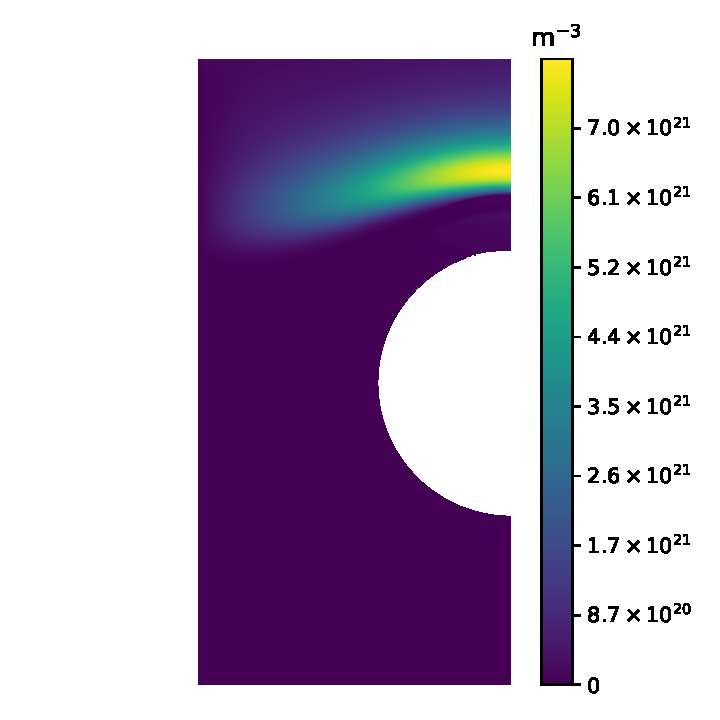
\includegraphics[width=\linewidth]{Figures/Chapter3/monoblocks/interface_condition/retention_chemical_pot_short_exposure.pdf}
        \caption{continuity of chemical potential.}
    \end{subfigure}%
    \begin{subfigure}{0.5\linewidth}
        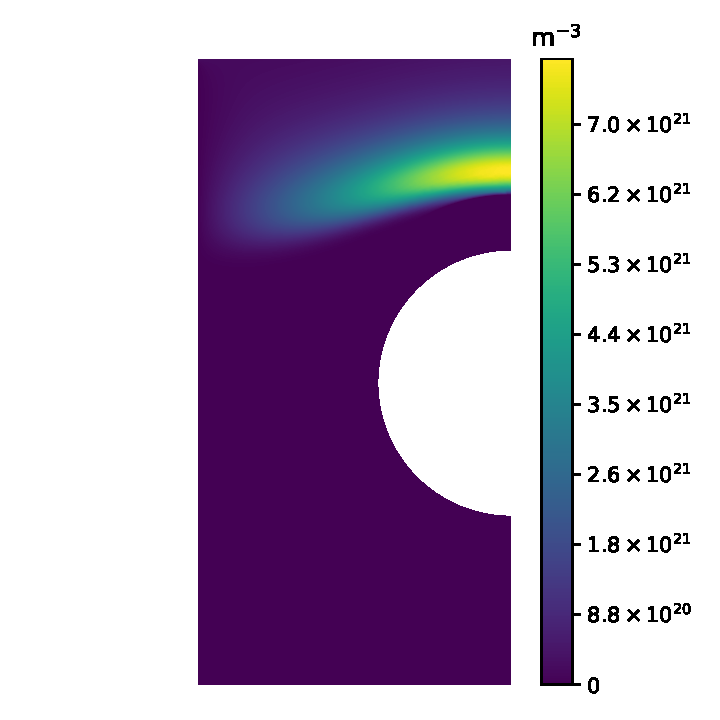
\includegraphics[width=\linewidth]{Figures/Chapter3/monoblocks/interface_condition/retention_concentration_short_exposure.pdf}
        \caption{continuity of mobile concentration.}
    \end{subfigure}
    \caption{Retention fields at $t=\SI{6.1e4}{s}$.}
    \labfig{retention fields w/wo chemical pot short exposure}
\end{figure}

Similarly, before reaching the W/Cu interface, the retention profiles are identical regardless of the interface condition (see \reffig{retention fields w/wo chemical pot short exposure}).

The retro-desorbed flux (from the monoblock to the plasma) does not depend on the interface conditions since interfaces are far from the exposed surface.
Moreover, outgassing flux through the cooling pipe greatly depends on the boundary condition imposed at the cooling surface.
Therefore, in order to assess the impact of interface conditions on the outgassing flux through the cooling pipe, uncertainties must first be lifted regarding the recombination process occurring on surfaces in contact with water.

Since this work is motivated by the estimation of the divertor inventory, the concentration continuity assumption is therefore valid since only a few monoblocks are exposed to high heat fluxes and most of the divertor is at the coolant temperature (this will be explained further in \refch{Divertor inventory estimation}).


\subsection{Influence of cycling}\labsec{influence of cycling}

In ITER, the plasma operation will not be continuous.
Instead, pulses of \SI{600}{s} will be shot \sidecite{lister_plasma_2006} with a ramp-up of \SI{100}{s}, a plateau during \SI{400}{s}, a ramp-down of \SI{100}{s} and \SI{1000}{s} of dwell time between pulses (see \reffig{plasma cycle}).
Simulating these transient cycles would require stepsizes of $\approx \SI{10}{s}$ in order to capture the ramp-up and ramp-down phases.
Simulating one cycle would therefore require more than 60 steps (excluding the resting phase).

On the other hand, FESTIM has an adaptive stepsize feature allowing the stepsize to increase (resp. decrease) when steps are solved in less (resp. more) than five Newton iterations.
Therefore, if a continuous plasma exposure was simulated, the adaptive stepsize would allow the stepsize to increase up to thousands of seconds, reducing a lot the simulation time.

To verify the validity of the continuous exposure approximation, 1D simulations were run with plasma cycles or continuous exposure.
For the cycled simulation, both the heat flux $\varphi_\mathrm{heat}$ and the particle flux $\varphi_\mathrm{imp}$ were varied from zero during the resting phases to their nominal values during the plateau phase (see \reffig{plasma cycle}).

Two cases were run:
\begin{itemize}
    \item High flux: $\varphi_\mathrm{heat} = \SI{13}{MW.m^{-2}}$ and $\varphi_\mathrm{imp} = \SI{1.6e22}{m^{-2}.s^{-1}}$
    \item Low flux: $\varphi_\mathrm{heat} = \SI{5}{MW.m^{-2}}$ and $\varphi_\mathrm{imp} = \SI{5.0e21}{m^{-2}.s^{-1}}$
\end{itemize}

In the high flux case, the surface temperature is about $\SI{1400}{K}$ during the plateau whereas it is only $\approx \SI{500}{K}$ for the low flux case.
The evolution of the inventory for both cases was calculated with or without cycling (see \reffig{monoblock inventory cycling}).
To be able to compare the cases, the inventory is shown as a function of the fluence:
\begin{equation}
    \mathrm{fluence}(t) = \int_0^t \varphi_\mathrm{imp}(t) \, dt
\end{equation}


\begin{figure}
    \centering
    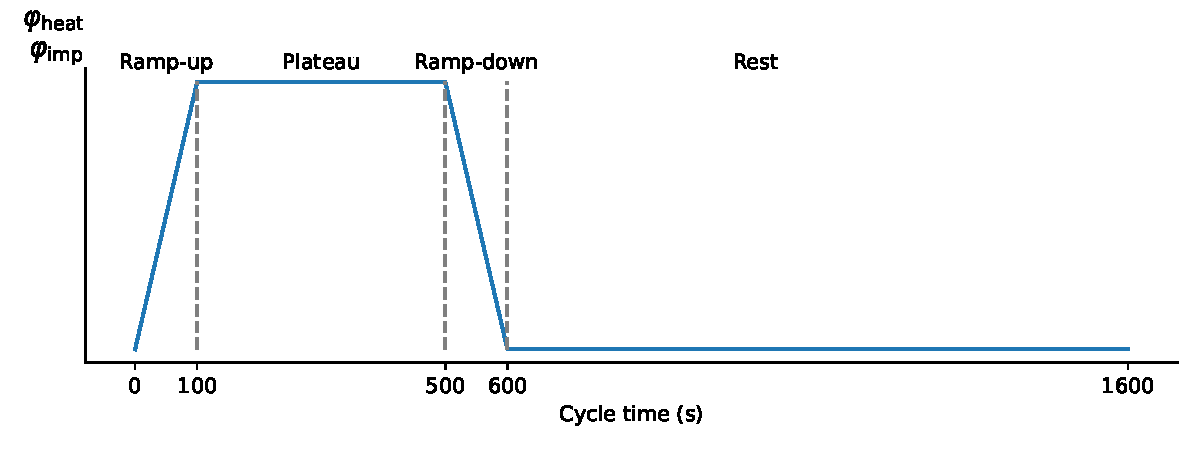
\includegraphics[width=\linewidth]{Figures/Chapter3/monoblocks/cycle.pdf}
    \caption{ITER plasma cycle. Evolution of heat flux and implanted particle flux.}
    \labfig{plasma cycle}
\end{figure}

\begin{figure}
    \centering
    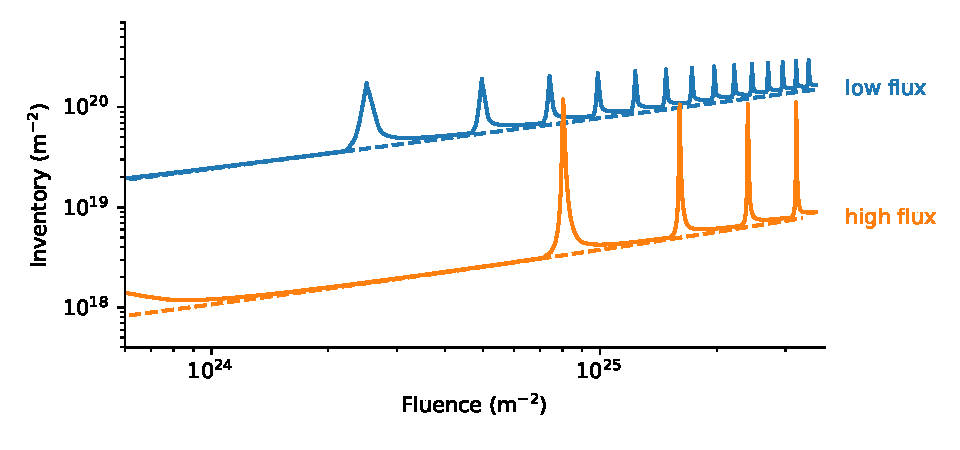
\includegraphics[width=\linewidth]{Figures/Chapter3/monoblocks/comparison_inventory_cycling.pdf}
    \caption{Evolution of the monoblock inventory as a function of the implanted fluence for cycled (solid) and continuous (dashed) exposure.}
    \labfig{monoblock inventory cycling}
\end{figure}

For the continuous cases, the inventory evolves as a power law of the fluence.
For the cycled simulations, spikes appear periodically (between every cycle).
These spikes correspond to ramp-down and ramp-ups during the cycles (see \reffig{monoblock inventory one cycle}).
During the ramp-down, as the temperature decreases, the traps filling ratio increases, which results in an increase in the inventory.
During the resting phase (not shown on \reffig{monoblock inventory cycling} since the flux is null), the inventory is kept constant.
During the ramp-up, the temperature increases again and the hydrogen trapped close to the plasma-facing surface is desorbed and diffuses either back to the plasma, or deeper into the bulk.
Finally, during the plateau phase, the inventory increases as a power law of the fluence.

\begin{figure}
    \centering
    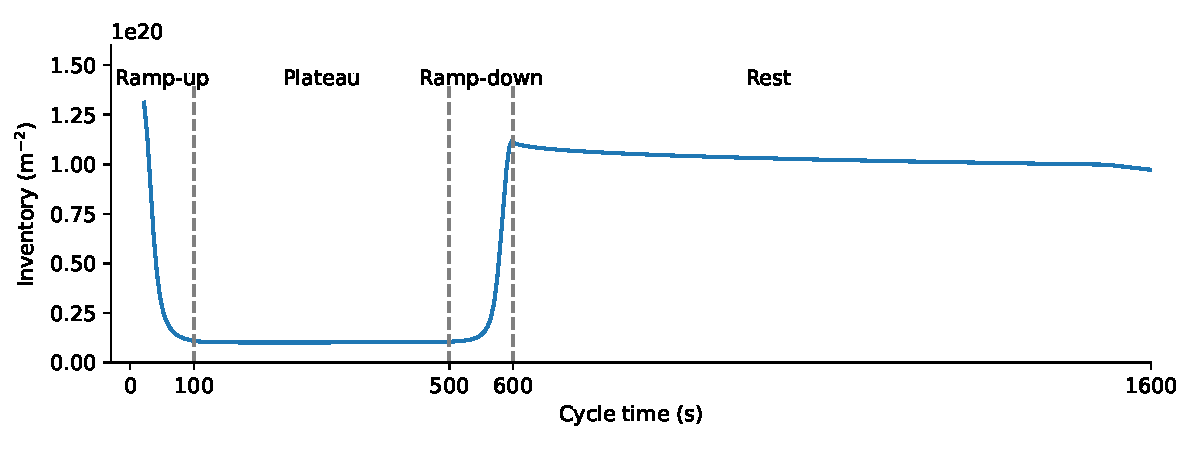
\includegraphics[width=\linewidth]{Figures/Chapter3/monoblocks/inventory_one_cycle.pdf}
    \caption{Evolution of the monoblock inventory during the sixth cycle for the high flux case.}
    \labfig{monoblock inventory one cycle}
\end{figure}

These kinetics are observed for both the low flux and high flux cases.
However, in the low flux case, the height of the spikes is greatly reduced.
This is explained by the lower temperature difference between the resting phase and the plateau phase.

In both cases, the evolution trends are the same with or without cycling and the inventory evolution during the plateau phases nearly match the continuous case.
These results are consistent with the one observed in \sidecite{hodille_modelling_2021} with other trapping parameters.
For a monoblock where the flux is even lower and the temperature difference is almost zero, no spikes will appear, and the cycled and continuous cases will match.

Moreover, the ``height'' of these spikes is constant.
This means that, after more cycles, these spikes will become negligible compared to the bulk inventory.
For the high flux case, the inventory spike will be negligible (10\% of the total inventory) after approximately 4000 cycles.
For the low flux case, it is negligible after only 1150 cycles.

This therefore validates the continuous exposure simplification.


\section{Monoblock behaviour law}\labsec{influence of exposure conditions}


\subsection{Simulation description}
The first step of the work was to simulate the hydrogenic transport and trapping in a tungsten monoblock as a function of the loading conditions.

Moreover, a parametric study will be carried out in order to simulate the whole range of the implantation conditions encountered in the ITER divertor.

% NO NEED TO PUT THE GEOMETRY HERE AGAIN
% \subsubsection{Geometry}
% The geometry used in this work is that of a non-shaped ITER monoblock (see Figure \ref{fig:monoblock geometry}).
% The monoblocks use tungsten armour and a \SI{1.5}{mm}-thick CuCrZr pipe as heat sink.
% The pipe is jointed to the tungsten.
% A \SI{1}{mm}-thick Cu interlayer is used in order to handle stress resulting from differential thermal expansion \sidecite{richou_realization_2017}.
% The surface $\Gamma_\mathrm{top}$ is facing the plasma and $\Gamma_\mathrm{coolant}$ is cooled by water.

% \begin{figure} [ht!]
%     \centering
%     \begin{overpic}[width=\linewidth]{Figures/Chapter3/monoblocks/parametric_study/monoblock_sketch.pdf}
%         \put(42, 5){\SI{28}{mm}}
%         \put(97, 50){\SI{28}{mm}}
%         \put(10, 32){\SI{13.5}{mm}}
%         \put(42, 62){ \diameter \SI{12}{mm}}
%         \put(42, 71){ \diameter \SI{15}{mm}}
%         \put(42, 78){ \diameter \SI{17}{mm}}
%         \put(20, 80){\large$\Gamma_\mathrm{top}$}
%         \put(40, 41){\large$\Gamma_\mathrm{coolant}$}
%     \end{overpic}
%     \caption{Monoblock geometry showing W armour \cruleme[grey]{0.3cm}{0.3cm}, Cu interlayer \cruleme[orange]{0.3cm}{0.3cm}, CuCrZr alloy cooling pipe  \cruleme[yellow]{0.3cm}{0.3cm}}
%     \label{fig:monoblock geometry}
% \end{figure}

% \subsubsection{Material properties}
% The material properties used in these simulations are described in Tables \ref{tab:materials properties_2} and their temperature dependence is shown in Figure \ref{fig:properties_2}.
% The trap parameters are described in Table \ref{tab:traps monoblock}.
% Influence of mechanical fields such as thermal expansion on trap creation \sidecite{benannoune_multidimensional_2020} was not taken into account in this work.
% Hodille \textit{et al} described an extrinsic trap in tungsten created by ion implantation \sidecite{hodille_macroscopic_2015}.
% This trap is assumed to have only a small influence on the macroscopic behaviour of the monoblock and is therefore not taken into account in this work for the sake of simplicity.

% \begin{table*}[ht]
%     \centering
%     \begin{tabular}{p{1.7cm}  R{3cm}  R{3cm}  R{1.8cm}  R{2.1cm} }
%          & \multicolumn{2}{c}{Thermal properties} & \multicolumn{2}{c}{Hydrogen transport}\\
%         \hline
%         Material & $\rho \cdot C_p \newline(\si{J.K^{-1}.m^{-3}})$ & $\lambda \newline(\si{W.m^{-1}.K^{-1}})$ & $D_0 \newline(\si{m^2.s^{-1}})$ & $E_\mathrm{diff} \newline(\si{eV})$\\
%         \hline
%         \\
%         W & %
%         $5.1\times 10^{-6} \cdot T^3 \newline - 8.3\times 10^{-2}\cdot T^2 \newline + 6.0 \times 10^{2}\cdot T \newline +2.4\times 10^6$ &%
%         $-7.8\times 10^{-9}\cdot T^3 \newline %
%         +5.0\times 10^{-5}\cdot T^2 \newline%
%         -1.1\times 10^{-1} \cdot T \newline%
%         +1.8\times 10^{2}$ &%
%         $1.9\times 10^{-7}$ & 0.20 \\
%         \\
%         Cu &%
%         $1.7\times 10^{-4}\cdot T^3\newline %
%         +6.1\times 10^{-2}\cdot T^2\newline %
%         +4.7\times 10^2\cdot T\newline %
%         +3.5\times 10^6$ &%

%         $-3.9\times 10^{-8}\cdot T^3\newline %
%         +3.8\times 10^{-5}\cdot T^2\newline %
%         -7.9\times 10^{-2}\cdot T\newline %
%         +4.0\times 10^2 $&%

%         $6.6\times 10^{-7}$ &%
%         0.39\\
%         \\
%         CuCrZr & %
%         $-1.8\times 10^{-4}\cdot T^3 \newline %
%         +1.5\times 10^{-1}\cdot T^2\newline %
%         +6.2\times 10^2\cdot T\newline %
%         +3.5\times 10^6$ &%

%         $5.3\times 10^{-7}\cdot T^3\newline %
%         -6.5\times 10^{-4}\cdot T^2\newline %
%         +2.6\times 10^{-1}\cdot T\newline %
%         +3.1\times 10^2$ & %

%         $3.9\times 10^{-7}$ & %
%         0.42\\
%         \\
%     \end{tabular}
%     \caption{Materials properties used in the simulations. Thermal properties are fitted from ANSYS. \cite{reiter_compilation_1996, serra_hydrogen_1998, fernandez_hydrogen_2015}}
%     \label{tab:materials properties_2}
% \end{table*}

% \begin{figure*} [h!]
%     \centering
%     \begin{subfigure}{0.5\linewidth}
%         \centering
%         \includegraphics[width=\linewidth]{Figures/Chapter3/monoblocks/parametric_study/thermal_prop.pdf}
%     \end{subfigure}%
%     \begin{subfigure}{0.5\linewidth}
%         \centering
%         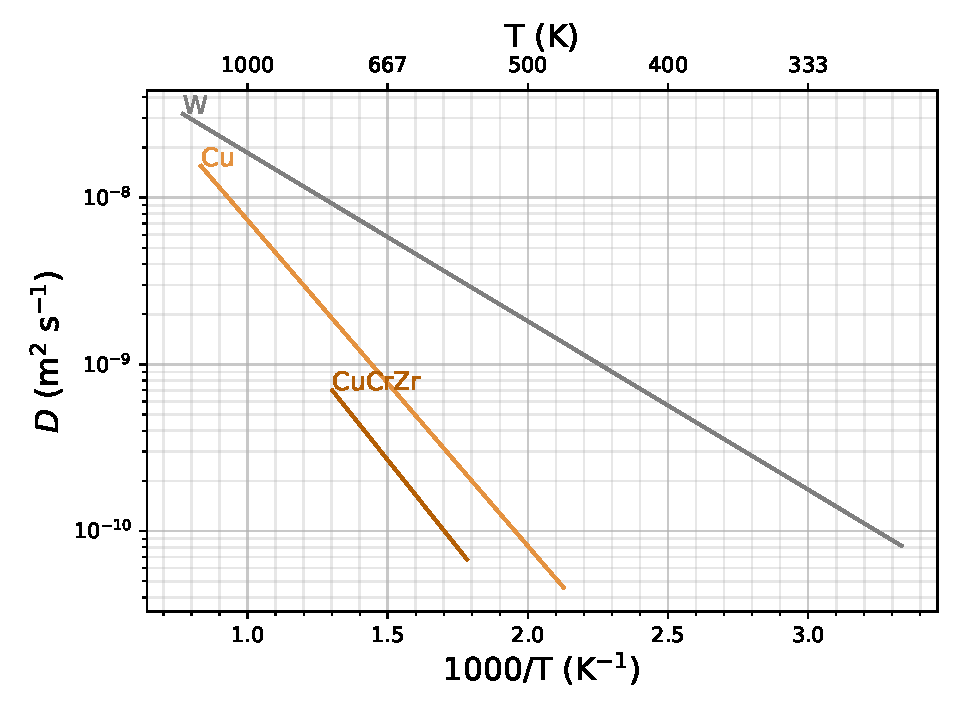
\includegraphics[width=\linewidth]{Figures/Chapter3/monoblocks/parametric_study/D_coeff.pdf}
%     \end{subfigure}
%     \caption{Material properties used in the simulations \cite{reiter_compilation_1996, serra_hydrogen_1998, fernandez_hydrogen_2015}}
%     \label{fig:properties_2}
% \end{figure*}

% \begin{table*} [ht]
%     \centering
%     \begin{tabular}{L{1.5cm} L{1.5cm} R{1.6cm} R{1.1cm} R{1.6cm} R{1.1cm} R{2cm}}
%          & Material & $k_0 (\si{m^3.s^{-1}})$ &  $E_k (\si{eV})$ & $p_0 (\si{s^{-1}})$ & $E_p (\si{eV})$ & $n_i (\si{at.fr.})$ \\
%         \hline
%         \\
%        Trap 1 & W & $3.1 \times 10^{-16}$ & 0.20 & $8.4 \times 10^{12}$& 1.00 & $1.1 \times 10^{-3}$ \\
%         \\
%         Trap 2 & Cu & $6.0 \times 10^{-17}$ & \textcolor{black}{0.39} & $8.0 \times 10^{13}$ & 0.50 &$5.0 \times 10^{-5}$\\
%         \\
%         Trap 3 & CuCrZr & $1.2 \times 10^{-16}$ & \textcolor{black}{0.42} & $8.0 \times 10^{13}$ & 0.85 &$5.0 \times 10^{-5}$\\
%         \\
%     \end{tabular}
%     \caption{Traps properties used in the simulations \cite{hodille_macroscopic_2015, dolan_assessment_1994}}
%     \label{tab:traps monoblock}
% \end{table*}

\subsubsection{Boundary conditions}

Mobile particles concentration $c_\mathrm{m}$ is imposed on $\Gamma_\mathrm{top}$ which allows to simulate particle implantation without having to include a volumetric source term applied on the first few nanometres.
This approximation allows to have a broader mesh and therefore saves computation time without affecting the macroscopic behaviour.
Molecular recombination is assumed on $\Gamma_\mathrm{coolant}$.
Even though it could be assumed on the gaps between monoblocks, it can be shown that its influence on the macroscopic behaviour remains low.
Desorption from the other surfaces is therefore assumed to be zero for simplification purposes.
\textcolor{black}{Uniform} heat loads $\varphi_H$ are applied on the surface $\Gamma_\mathrm{top}$ with a Neumman boundary condition or temperature is constrained on $\Gamma_\mathrm{top}$ with a Dirichlet boundary condition and a convective exchange condition is set on surface $\Gamma_\mathrm{coolant}$.
All the other surfaces are assumed thermally insulated.
The set of boundary conditions can finally be described as follow:

\begin{subequations}
    \begin{align}
    -\lambda \vec{\nabla} T \cdot \vec{n} &=\varphi_{H} \quad \text{or} \quad T = T_\mathrm{surface}\quad &\text { on } \Gamma_\mathrm{top}\\
    c_\mathrm{m} &=  c_\mathrm{surface}\quad &\text { on } \Gamma_\mathrm{top}\\
    -\lambda \vec{\nabla} T\cdot \vec{n} &= -h \cdot \left(T_\mathrm{coolant} - T\right)\quad &\text { on } \Gamma_\mathrm{coolant}\\
    -D \vec{\nabla} c_\mathrm{m} \cdot \vec{n} &= K_\mathrm{CuCrZr} \cdot c_\mathrm{m}^{2} \quad &\text { on } \Gamma_\mathrm{coolant}
    \end{align}
\end{subequations}
with $h=\SI{70000}{W.m^{-2}.K^{-1}}$ being the heat exchange coefficient calculated from the Sieder-Tate correlation for the forced convection regime, $T_\mathrm{coolant}= \SI{323}{K}$ and $\vec{n}$ the normal vector and $K_\mathrm{CuCrZr} = 2.9 \times 10^{-14}\cdot \exp{(-1.92/(k_B\cdot T))}$ the recombination coefficient of the copper alloy (in vacuum) expressed in \si{m^4.s^{-1}} \sidecite{anderl_deuterium_1999}.

% The thermal response of ITER-like monoblocks to the heat load $\varphi_H$ has first been studied.
% Then the hydrogen inventory was determined as a function of surface temperature and surface concentration and as a function of the implanted particle flux and the incident ion energy.
% Finally, an application on ITER exposure conditions was made.

\subsection{Thermal behaviour}
Steady-state heat transfer simulations were performed with FESTIM with varying heat loads $\varphi_H$.
With $\varphi_H = \SI{1}{MW.m^{-2}}$, the surface temperature of the monoblock was found to be around \SI{400}{K} (see Figure \ref{fig:T field 1 MW}) whereas with $\varphi_H = \SI{10}{MW.m^{-2}}$ the surface was around \SI{1400}{K} (see Figure \ref{fig:T field 10 MW}).

\begin{figure*} [h!]
    \centering
    \begin{subfigure}{0.4\linewidth}
        \centering
        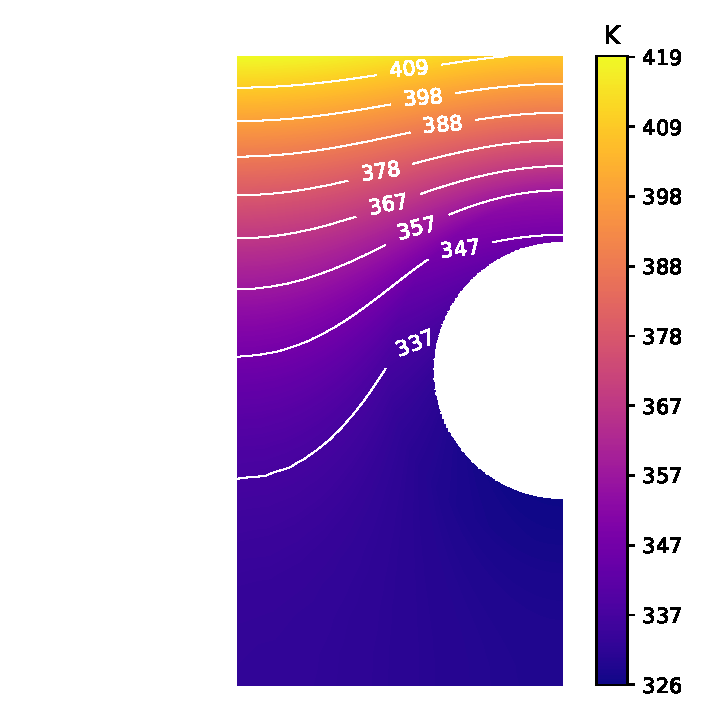
\includegraphics[width=\linewidth]{Figures/Chapter3/monoblocks/parametric_study/T_1e6.pdf}
        \caption{Temperature field with $\varphi_H = \SI{1}{MW.m^{-2}}$}
        \label{fig:T field 1 MW}
    \end{subfigure}%
    \begin{subfigure}{0.4\linewidth}
        \centering
        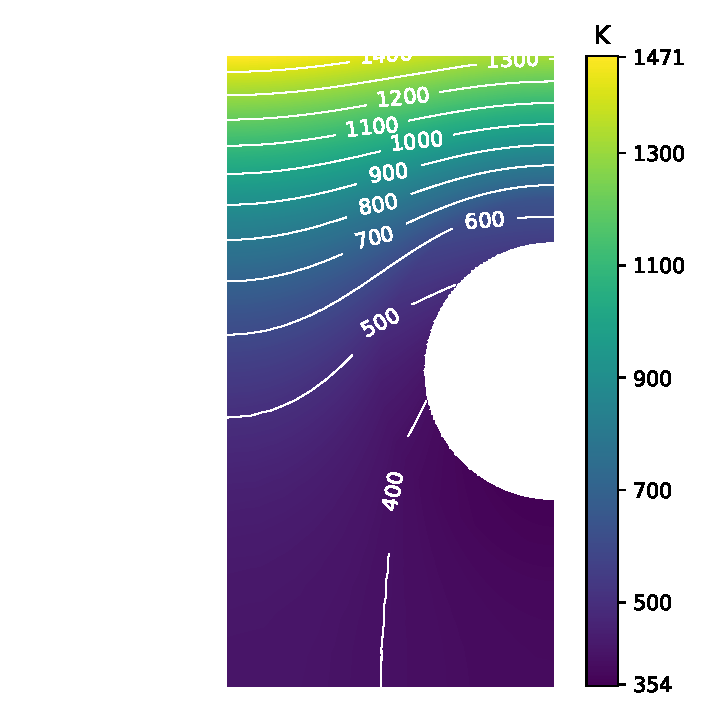
\includegraphics[width=\linewidth]{Figures/Chapter3/monoblocks/parametric_study/T_1e7.pdf}
        \caption{Temperature field with $\varphi_H = \SI{10}{MW.m^{-2}}$}
        \label{fig:T field 10 MW}
    \end{subfigure}
    \begin{subfigure}{0.7\linewidth}
        \centering
        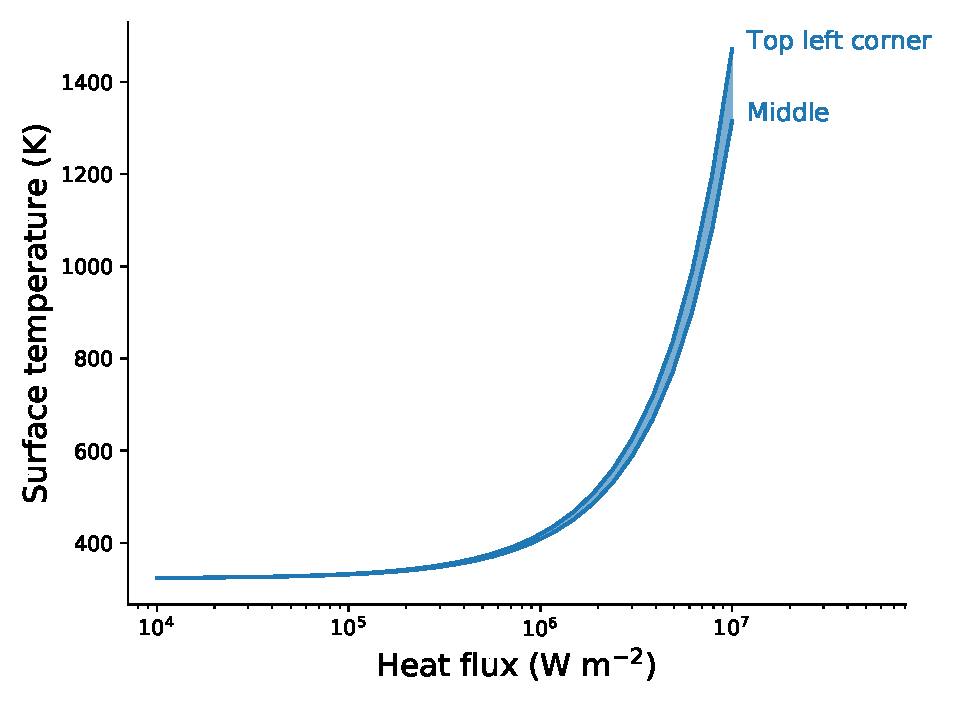
\includegraphics[width=\linewidth]{Figures/Chapter3/monoblocks/parametric_study/temperature_phi_H.pdf}
        \caption{\textcolor{black}{Evolution of surface temperature as a function of heat flux}}
        \label{fig:T phi_H}
    \end{subfigure}
    \caption{Thermal behaviour of the monoblock}
\end{figure*}

$T_\mathrm{surface}$ \textcolor{black}{therefore} increases linearly with the heat load and can be modelled by Equation \ref{eq:thermal behaviour law} (see Figure \ref{fig:T phi_H}).
\begin{equation}
    T_\mathrm{surface} = 1.1 \times 10^{-4} \cdot \varphi_H + T_\mathrm{coolant}
    \label{eq:thermal behaviour law}
\end{equation}

This was found to be in very good agreement with experimental measurements performed in \sidecite{hirai_use_2016}.

\subsection{Influence of \texorpdfstring{$T_\mathrm{surface}$}{Tsurface} and \texorpdfstring{$c_\mathrm{surface}$}{csurface} on hydrogen inventory}

In this section, the total inventory of hydrogen in monoblocks has been calculated as a function of $T_\mathrm{surface}$ and $c_\mathrm{surface}$.
Temperature and mobile concentration of hydrogen were imposed with Dirichlet boundary conditions on $\Gamma_\mathrm{top}$ with $T_\mathrm{surface}$ varying from $T_\mathrm{coolant}$ to \SI{1200}{K} and $c_\mathrm{surface}$ varying \textcolor{black}{arbitrarily} from \SI{e20}{m^{-3}} to \SI{6e22}{m^{-3}}.
The assumption of a constant surface temperature had low influence on the results compared to a non-homogeneous surface temperature that could be obtained with a heat flux condition since surface temperature gradient was low compared to the one between the top surface and the cooling surface.
For surface temperatures below \SI{500}{K}, 1D simulations were performed for the penetration depth of hydrogen remained very low (a few microns) and 1D approximation was sufficient \sidecite{benannoune_numerical_2019}.
For temperatures above \SI{500}{K} for which edge effects become dominant, 2D simulations have been performed.

After $ \SI{e7}{s}$ a high retention zone appeared far from the exposed surface $\Gamma_\mathrm{top}$ (see Figure \ref{fig:retention fields}).
As described in \sidecite{delaporte-mathurin_finite_2019}, this is due to thermal effects.
As seen in Figures \ref{fig:T field 1 MW} and \ref{fig:T field 10 MW}, the temperature was found to decrease in regions close to the cooling pipe $\Gamma_\mathrm{coolant}$ leading to an increase in trap occupancy, creating this high retention zone.
This was however not true for monoblocks where $T_\mathrm{surface} \approx T_\mathrm{coolant}$ since the temperature gradient in the domain is very low.
Instead, trap occupancy was close to one and the retention was high in the whole region where hydrogen had penetrated and not only far from the top surface.

\begin{figure*}
    \centering
    \begin{subfigure}{0.5\linewidth}
        \centering
        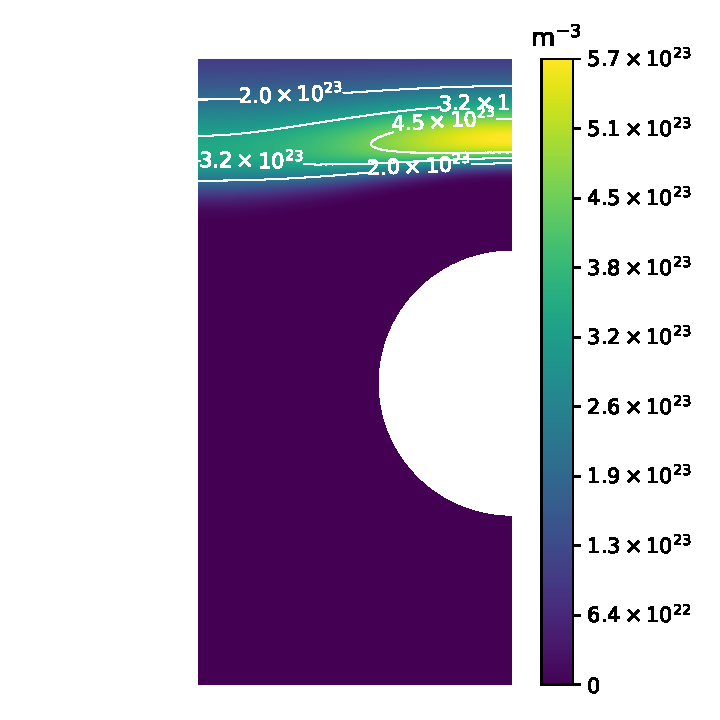
\includegraphics[height=\linewidth]{Figures/Chapter3/monoblocks/parametric_study/retention_T=7.000e+02;c=1.00e+20.pdf}
        \caption{$T_\mathrm{surface} = \SI{700}{K}$ and $c_\mathrm{surface} = \SI{e20}{m^{-3}}$}
    \end{subfigure}%
    \begin{subfigure}{0.5\linewidth}
        \centering
        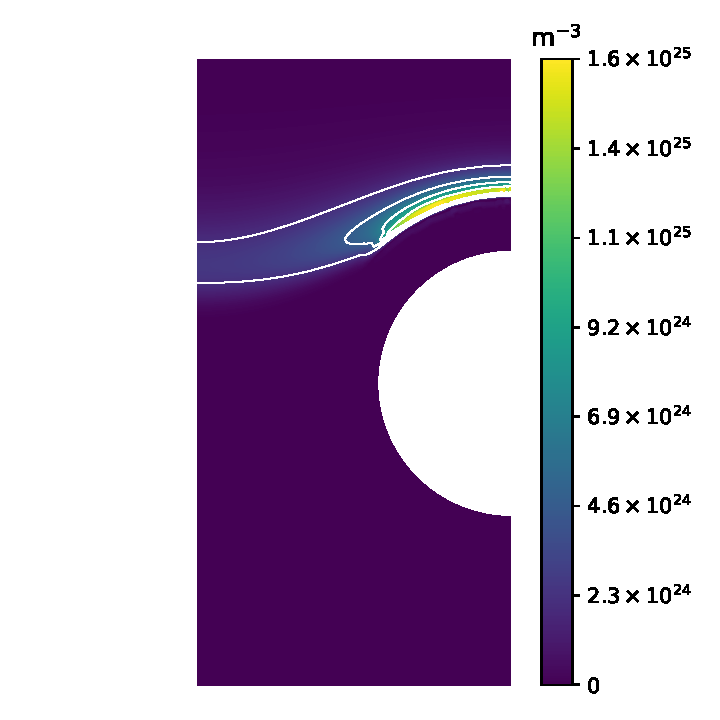
\includegraphics[height=\linewidth]{Figures/Chapter3/monoblocks/parametric_study/retention_T=1.000e+03;c=1.00e+21.pdf}
        \caption{$T_\mathrm{surface} = \SI{1000}{K}$ and $c_\mathrm{surface} = \SI{e21}{m^{-3}}$}
    \end{subfigure}
    \caption{Retention fields in \si{m^{-3}} after a \SI{e7}{s} exposure}
    \label{fig:retention fields}
\end{figure*}


Hydrogen inventory in monoblocks as a function of $T_\mathrm{surface}$ and $c_\mathrm{surface}$ is shown in Figure \ref{fig:inventory T c}.
In order to obtain this continuous field, more than 600 simulations randomly distributed on the parameter plane were run and analysed using a Gaussian process machine learning algorithm \sidecite{rasmussen_gaussian_2006} as in \sidecite{shimwell_multiphysics_2019} based on the python package inference-tools \sidecite{chris_bowman_c-bowmaninference-tools_2020}.
In Figure \ref{fig:inventory T c}, the inventory obtained by the Gaussian regression process is given for a constant value of $c_\mathrm{surf}=\SI{2e21}{m^{-3}}$ (top inset) and a constant temperature $T=\SI{850}{K}$ (left inset).
The Gaussian regression process was particularly appropriate as it calculates a confidence interval based on the standard deviation $\sigma$.
As expected, the lower the density of simulation points, the higher was the value of $\sigma$ (for example around \SI{850}{K} on the top inset of Figure \ref{fig:inventory T c}).
However, despite the lack of simulation in this region, the value of $\sigma$ was still acceptable (only a few percents of the inventory) ensuring the quality of the resulting interpolation.

As expected, inventory was found to globally increase with $c_\mathrm{surface}$.
For $T_\mathrm{surface} > \SI{550}{K}$, the inventory tended to decrease with surface temperature.
However, for $T_\mathrm{surface} < \SI{550}{K}$, inventory increased with surface temperature.
This phenomenon is due to a trade-off between an increase of the detrapping rate and an increase of the diffusion coefficient making the hydrogen particles penetrate deeper into the bulk.
Above $\SI{550}{K}$, detrapping becomes dominant and inventory decreases.
This mapping of inventory as a function of $T_\mathrm{surface}$ and $c_\mathrm{surface}$ provides an easy way of estimating the inventory in monoblocks for several exposure conditions without having to run many simulations.
Indeed, to estimate the inventory with different exposure conditions, one only needs to associate these conditions $(\varphi_\mathrm{inc}, E)$ to a couple $(c_\mathrm{surf}, T_\mathrm{surf})$.

\begin{figure*} [h]
    \centering
    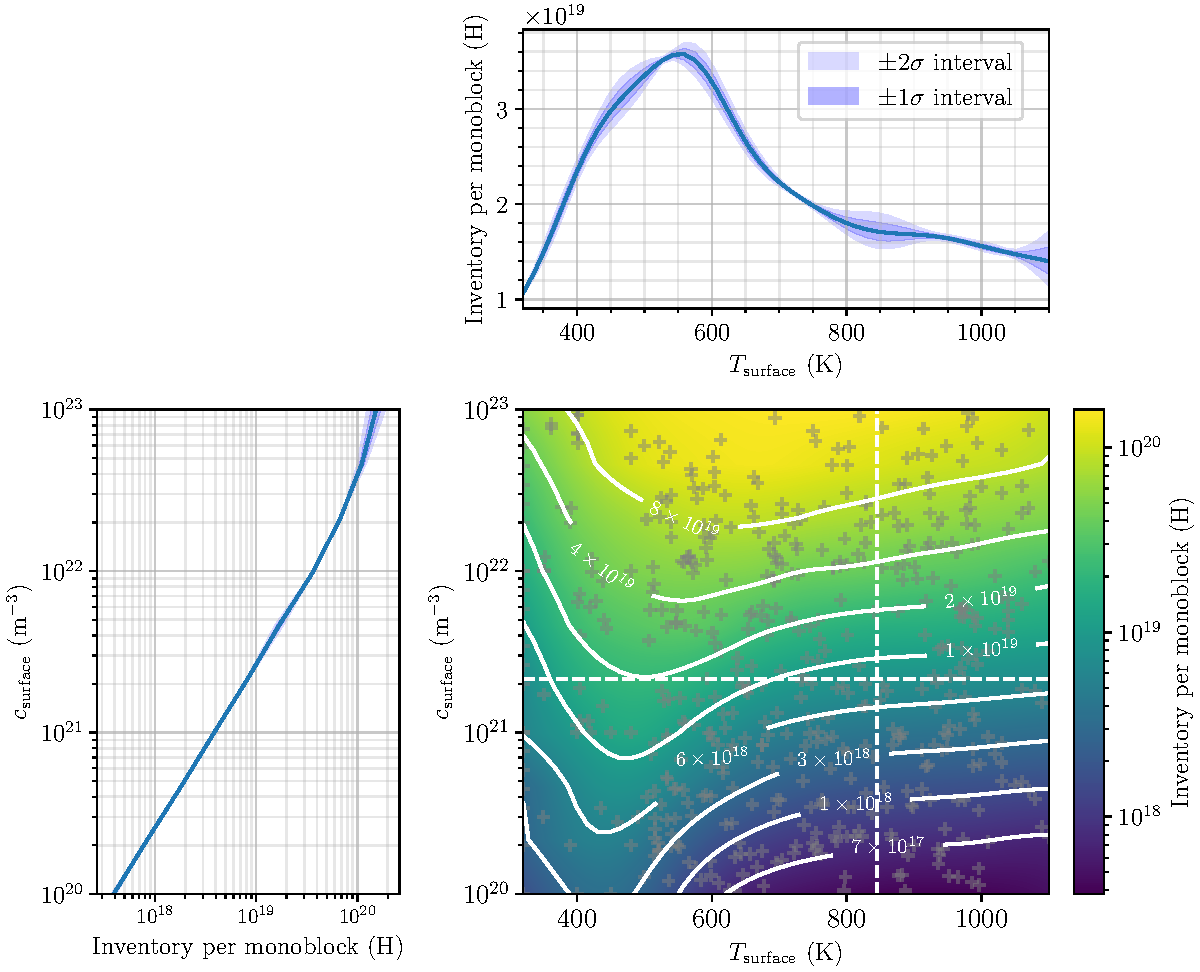
\includegraphics[width=\linewidth]{Figures/Chapter3/monoblocks/parametric_study/inventory_T_c_profiles.pdf}
    \caption{Evolution of the inventory after a \SI{e7}{s} exposure as a function of $T_\mathrm{surface}$ and $c_\mathrm{surface}$ alongside with simulation points (grey crosses). The simulations points were fitted with a Gaussian regression process \cite{chris_bowman_c-bowmaninference-tools_2020} providing the standard deviation $\sigma$.}
    \label{fig:inventory T c}
\end{figure*}

\subsection{Discussion}
If this methodology provides a rapid way of estimating hydrogen content in the whole divertor, several assumptions have however been made.


% Influence of cycling
First, a steady state exposure was considered for simplification purposes.
This result is however conservative.
As seen in \sidecite{delaporte-mathurin_finite_2019, hodille_estimation_2017}, cycling effects could have an influence in regions where $T_\mathrm{surface}$ varies a lot, for example \textcolor{black}{within \SI{10}{cm} on both sides of the strike points}.
Though, since a large majority of monoblocks stay at room temperature, even during operations the thermal effect should remain low and discrepancies would rather be due to particle flux evolution along the target.

% shaping
Shaping of monoblocks (\textit{e.g.} chamfers) was not taken into account in this work for simplification purposes.
Such shaping can have an influence on the incident particle and heat loads on the plasma facing surface of the monoblocks.



% Be deposits
This study presents the hydrogen trapping in W monoblocks.
It shows that the latter remains low but, as already pointed out by JET studies, the trapping on Be co-deposited layers is expected to be the main mechanism for tritium retention in ITER \sidecite{brezinsek_beryllium_2015, heinola_fuel_2015}.
Such layers could be found in the cold regions of the divertor but as soon as the strike points hit these layers, they should be sputtered away (as sputtering of Be is possible even at low energy \sidecite{bjorkas_variables_2013} \cite{brezinsek_beryllium_2015}).
The retention where the deposited layers are not present (either sputtered or not formed anyway) would then be given by the model presented here.

% Coolant recombination
The molecular recombination coefficient at the surface of the cooling pipe was taken from \sidecite{anderl_deuterium_1999} and was measured in vacuum.
One could argue that recombination in presence of water will be facilitated.
It can however be shown that this parameter has very low influence on the inventory since it was dominated by retention in tungsten.
This parameter will however have an influence on the permeation flux and should be studied in future work.

% Gap recombination
\textcolor{black}{Similarly, the influence on molecular recombination on the sides of the monoblock was found to have a low impact on the results.
By assuming an instantaneous recombination coefficient, the relative error on the monoblock inventory was found to be significant only in hot regions (\textit{ie} within \SI{10}{cm} on both sides of the strike points).
The influence on the total divertor inventory is therefore low (less than \SI{5}{\%} after a \SI{e7}{s} exposure) since it is dominated by regions where $T_\mathrm{surface} \approx T_\mathrm{coolant}$.}

% ELMs
It should be noted that specific scenarii like edge localised modes (ELMs) were also not taken into account in this work since their time scale is very short.
MRE simulations by Hu and Hassanein \sidecite{hu_predicting_2015} suggest that a \SI{400}{s} discharge with \SI{1}{Hz} or \SI{10}{Hz} ELMs significantly reduces (77 \%) the inventory in W materials.
However, the modelling of the ELM is simulated by increasing the temperature for a very short time without changing the incident flux of particles that can also be much higher thus balancing the fuel retention reduction.
Another study by Schmid \textit{et al} \sidecite{schmid_diffusion-trapping_2016} also simulated the effect of \SI{1}{Hz} ELMs on fuel retention in W.
The outcome is that \SI{6}{s} of \SI{1}{Hz}-ELMs does not affect significantly the fuel retention, though the temperature excursion in those simulations are smaller than for the one of Hu and Hassanein.
Thus, the effect of ELMs, especially the balance between increase of heat flux, incident energy and particle flux, could either favour or disfavour trapping, diffusion and migration and therefore the overall retention.

% Surface process
In this study the model to link the concentration of mobile particles at the surface (implantation zone) with the exposure condition considers that the particles are implanted in the bulk and that the recombination coefficient is very high since many uncertainties concerning the recombination coefficient are yet to be lifted.
However, if an exothermic process is considered as in \sidecite{ogorodnikova_recombination_2019}, this should have low influence since recombination is very quick at a temperature close to that of the coolant.

On the other hand, experimental results \sidecite{t_hoen_strongly_2013} suggest that for ion energy below \SI{5}{eV/H}, typical of detached plasma as the one treated in the previous section, the surface process can be important and limits the uptake of hydrogen, i.e. the adsorption on the surface and the further absorption from surface to bulk could be the limiting process for the growth of $c_\mathrm{surface}$ during such exposure.
The evolution of $c_\mathrm{surface}$ to the exposure condition for that range of energy would therefore be different and therefore the inventory.
The advantage of the presented method is that taking into account such process is realtively easy as no expensive simulations are needed.
One would only need to modify the model giving $c_\mathrm{surface}$
as a function of $(E_\mathrm{inc},\varphi_\mathrm{inc})$ to include the different surface processes.
To this end, one can use kinetic surface models \sidecite{hodille_retention_2017, zaloznik_deuterium_2017, pecovnik_influence_2019, guterl_effects_2019}.

% traps
Trap properties have a great impact on the inventory.
In this study, a homogeneous trap distribution is assumed for simplification purposes.
A more thorough study could investigate the influence on trap distribution, energy and density.
Trap properties might also vary along the divertor based on exposure conditions.
Moreover the impact of neutrons must be assessed as neutron-induced traps have a high detrapping energy.


% Helium

Finally, helium implantation in the materials and bubble formation could modify the hydrogen transport in monoblocks.

\subsection{Summary}
ITER-like monoblocks have been studied using a novel method in order to estimate the hydrogen content as a function of exposure conditions such as the implanted particle flux, the ion energy, the heat load and the monoblock surface temperature.
Several hundred data points have been simulated with FESTIM and analysed to estimate the hydrogen inventory in monoblocks for any input conditions using a Gaussian regression process, a machine learning algorithm which calculates the confidence interval for each point.
Thanks to this relation, one can easily estimate hydrogen content in the whole divertor without having to run all the simulations.
An application has been made based on the output from a SOLPS calculation of exposure conditions distribution on the ITER divertor and shows that for these conditions the inventory could reach \SI{e20}{H} per monoblock near strike points after a \SI{e7}{s} exposure.
The total hydrogen content in ITER divertor is estimated to be \SI{8}{g} which is well below the inner-vessel safety limit of \SI{1}{kg}.

This behaviour law will be used in \refch{Divertor inventory estimation} to estimate the hydrogen inventory of WEST and ITER divertors.

\section{Summary}
H transport in ITER-like monoblocks was simulated with FESTIM.

The validity of various simplifications and assumptions was first studied.
A relationship between the average surface temperature and the heat flux was obtained.
It was then shown that the choice of interface conditions (continuity of chemical potential or continuity of mobile concentration) had low impact on the monoblock inventory.
Moreover, the 2D approximation was found to be the best compromise between accuracy of the solution and computational time.
The effect of loading cycles was also investigated.
Between plasma pulses, a zone with higher retention appears near the plasma exposed surface due to the temperature variation.
These modifications of the retention fields vanish as soon as the next cycle starts again and this zone is heated up again.
This means that cycling has no effect on the global retention field and that cycles can safely be concatenated (continuous exposure) to simulate H transport.

A parametric study was then performed in order to assess the influence of exposure conditions (surface concentration and surface temperature).
A behaviour law was obtained correlating exposure conditions to the monoblock inventory at a given exposure time.
This law will be extremely useful to estimate H retention in divertors in \refch{Divertor inventory estimation} since not all monoblocks will be exposed to the same exposure.
